\documentclass{article}
\usepackage{amsmath,amsfonts,amssymb,amsthm}
\usepackage{natbib}
\usepackage{booktabs}
\usepackage{xcolor}
\usepackage{paralist}
\usepackage{xspace}
\usepackage{graphicx}
%\usepackage{ulem}  % this underlines titles in the references so we should comment it out before the final version

\newtheorem{theorem}{Theorem}

\newcommand{\art}[1]{\begingroup\color{blue}#1\endgroup}
\newcommand{\aadit}[1]{\begingroup\color{orange}#1\endgroup}
\newcommand{\fred}[1]{\begingroup\color{red}#1\endgroup}
\newcommand{\alexei}[1]{\begingroup\color{green}#1\endgroup}

% Lets make it look like writing on a blackboards
% not a 1970s typewriter!
\renewcommand{\le}{\leqslant}
\renewcommand{\ge}{\geqslant}
\renewcommand{\leq}{\leqslant}
\renewcommand{\geq}{\geqslant}
\renewcommand{\emptyset}{\varnothing}

\DeclareSymbolFont{GreekLetters}{OML}{cmr}{m}{it} %Provide missing letters
\DeclareSymbolFont{UpSfGreekLetters}{U}{cmss}{m}{n} %Provide missing letters
\DeclareMathSymbol{\varrho}{\mathalpha}{GreekLetters}{"25}
\DeclareMathSymbol{\UpSfLambda}{\mathalpha}{UpSfGreekLetters}{"03}
\DeclareMathSymbol{\UpSfSigma}{\mathalpha}{UpSfGreekLetters}{"06}
%\newcommand{\bvec}[1]{\boldsymbol{#1}}
\providecommand{\mathbold}{\boldsymbol}
\newcommand{\bvec}[1]{\mathbold{#1}}
%\newcommand{\bvec}[1]{\text{\boldmath$#1$}}
\newcommand{\avec}[1]{\vec{#1}}
%\renewcommand{\vec}[1] {\text{\boldmath$#1$}}
%\renewcommand{\vec}[1]{\ensuremath{\mathbf{#1}}}
%\newcommand{\vecsym}[1]{\ensuremath{\boldsymbol{#1}}}
\newcommand{\vecsym}[1]{\ensuremath{\mathbold{#1}}}
\def\bbl{\text{\boldmath$\{$}}
\def\bbr{\text{\boldmath$\}$}}
\newcommand{\bbrace}[1]{\bbl #1 \bbr}
\newcommand{\bbbrace}[1]{\mathopen{\pmb{\bigg\{}}#1\mathclose{\pmb{\bigg\}}}}
\def\betahat{\hat\beta}
\newcommand{\dif}{{\rm d}}

\newlength{\overwdth}
\def\overstrike#1{ 
\settowidth{\overwdth}{#1}\makebox[0pt][l]{\rule[0.5ex]{\overwdth}{0.1ex}}#1}

\makeatletter
\newcommand*\bigcdot{\mathpalette\bigcdot@{.7}}
\newcommand*\bigcdot@[2]{\mathbin{\vcenter{\hbox{\scalebox{#2}{$\m@th#1\bullet$}}}}}
\makeatother

\def\abs#1{\ensuremath{\left \lvert #1 \right \rvert}}
\newcommand{\normabs}[1]{\ensuremath{\lvert #1 \rvert}}
\newcommand{\bigabs}[1]{\ensuremath{\bigl \lvert #1 \bigr \rvert}}
\newcommand{\Bigabs}[1]{\ensuremath{\Bigl \lvert #1 \Bigr \rvert}}
\newcommand{\biggabs}[1]{\ensuremath{\biggl \lvert #1 \biggr \rvert}}
\newcommand{\Biggabs}[1]{\ensuremath{\Biggl \lvert #1 \Biggr \rvert}}
\newcommand{\norm}[2][{}]{\ensuremath{\left \lVert #2 \right \rVert}_{#1}}
\newcommand{\normnorm}[2][{}]{\ensuremath{\lVert #2 \rVert}_{#1}}
\newcommand{\bignorm}[2][{}]{\ensuremath{\bigl \lVert #2 \bigr \rVert}_{#1}}
\newcommand{\Bignorm}[2][{}]{\ensuremath{\Bigl \lVert #2 \Bigr \rVert}_{#1}}
\newcommand{\biggnorm}[2][{}]{\ensuremath{\biggl \lVert #2 \biggr \rVert}_{#1}}
\newcommand{\Biggnorm}[2][{}]{\ensuremath{\Biggl \lVert #2 \Biggr \rVert}_{#1}}
\newcommand{\ip}[3][{}]{\ensuremath{\left \langle #2, #3 \right \rangle_{#1}}}

\newcommand{\bigvecpar}[3]{\ensuremath{\bigl ( #1 \bigr )_{#2}^{#3}}}
\newcommand{\Bigvecpar}[3]{\ensuremath{\Bigl ( #1 \Bigr )_{#2}^{#3}}}
\newcommand{\biggvecpar}[3]{\ensuremath{\biggl ( #1 \biggr )_{#2}^{#3}}}
\newcommand{\bigpar}[1]{\ensuremath{\bigl ( #1 \bigr )}}
\newcommand{\Bigpar}[1]{\ensuremath{\Bigl ( #1 \Bigr )}}
\newcommand{\biggpar}[1]{\ensuremath{\biggl ( #1 \biggr )}}

\newcommand{\IIDsim}{\overset{\textup{IID}}{\sim}}
\newcommand{\LDsim}{\overset{\textup{LD}}{\sim}}

\DeclareMathOperator{\success}{succ}
\DeclareMathOperator{\sinc}{sinc}
\DeclareMathOperator{\sech}{sech}
\DeclareMathOperator{\csch}{csch}
\DeclareMathOperator{\dist}{dist}
\DeclareMathOperator{\spn}{span}
\DeclareMathOperator{\sgn}{sgn}
\DeclareMathOperator*{\rmse}{rmse}
\DeclareMathOperator{\Prob}{\mathbb{P}}
\DeclareMathOperator{\Ex}{\mathbb{E}}
\DeclareMathOperator{\rank}{rank}
\DeclareMathOperator{\erfc}{erfc}
\DeclareMathOperator{\erf}{erf}
\DeclareMathOperator{\cov}{cov}
\DeclareMathOperator{\cost}{cost}
\DeclareMathOperator{\comp}{comp}
\DeclareMathOperator{\corr}{corr}
\DeclareMathOperator{\diag}{diag}
\DeclareMathOperator{\var}{var}
\DeclareMathOperator{\opt}{opt}
\DeclareMathOperator{\brandnew}{new}
\DeclareMathOperator{\std}{std}
\DeclareMathOperator{\kurt}{kurt}
\DeclareMathOperator{\med}{med}
\DeclareMathOperator{\vol}{vol}
\DeclareMathOperator{\bias}{bias}
\DeclareMathOperator*{\argmax}{argmax}
\DeclareMathOperator*{\argmin}{argmin}
\DeclareMathOperator{\sign}{sign}
\DeclareMathOperator{\spann}{span}
\DeclareMathOperator{\cond}{cond}
\DeclareMathOperator{\trace}{trace}
\DeclareMathOperator{\Si}{Si}
%\DeclareMathOperator{\diag}{diag}
\DeclareMathOperator{\col}{col}
\DeclareMathOperator{\nullspace}{null}
\DeclareMathOperator{\Order}{{\mathcal O}}
%\DeclareMathOperator{\rank}{rank}

\newcommand{\vzero}{\bvec{0}}
\newcommand{\vone}{\bvec{1}}
\newcommand{\vinf}{\bvec{\infty}}
\newcommand{\va}{\bvec{a}}
\newcommand{\vA}{\bvec{A}}
\newcommand{\vb}{\bvec{b}}
\newcommand{\vB}{\bvec{B}}
\newcommand{\vc}{\bvec{c}}
\newcommand{\vC}{\bvec{C}}
\newcommand{\vd}{\bvec{d}}
\newcommand{\vD}{\bvec{D}}
\newcommand{\ve}{\bvec{e}}
\newcommand{\vf}{\bvec{f}}
\newcommand{\vF}{\bvec{F}}
\newcommand{\vg}{\bvec{g}}
\newcommand{\vG}{\bvec{G}}
\newcommand{\vh}{\bvec{h}}
\newcommand{\vH}{\bvec{H}}
\newcommand{\vi}{\bvec{i}}
\newcommand{\vj}{\bvec{j}}
\newcommand{\vk}{\bvec{k}}
\newcommand{\vK}{\bvec{K}}
\newcommand{\vl}{\bvec{l}}
\newcommand{\vell}{\bvec{\ell}}
\newcommand{\vL}{\bvec{L}}
\newcommand{\vm}{\bvec{m}}
\newcommand{\vp}{\bvec{p}}
\newcommand{\vq}{\bvec{q}}
\newcommand{\vr}{\bvec{r}}
\newcommand{\vs}{\bvec{s}}
\newcommand{\vS}{\bvec{S}}
\newcommand{\vt}{\bvec{t}}
\newcommand{\vT}{\bvec{T}}
\newcommand{\vu}{\bvec{u}}
\newcommand{\vU}{\bvec{U}}
\newcommand{\vv}{\bvec{v}}
\newcommand{\vV}{\bvec{V}}
\newcommand{\vw}{\bvec{w}}
\newcommand{\vW}{\bvec{W}}
\newcommand{\vx}{\bvec{x}}
\newcommand{\vX}{\bvec{X}}
\newcommand{\vy}{\bvec{y}}
\newcommand{\vY}{\bvec{Y}}
\newcommand{\vz}{\bvec{z}}
\newcommand{\vZ}{\bvec{Z}}

\newcommand{\ai}{\avec{\imath}}
\newcommand{\ak}{\avec{k}}
\newcommand{\avi}{\avec{\bvec{\imath}}}
\newcommand{\at}{\avec{t}}
\newcommand{\avt}{\avec{\vt}}
\newcommand{\ax}{\avec{x}}
\newcommand{\ah}{\avec{h}}
\newcommand{\akappa}{\avec{\kappa}}
\newcommand{\avx}{\avec{\vx}}
\newcommand{\ay}{\avec{y}}
\newcommand{\avy}{\avec{\vy}}
\newcommand{\avz}{\avec{\vz}}
\newcommand{\avzero}{\avec{\vzero}}
\newcommand{\aomega}{\avec{\omega}}
\newcommand{\avomega}{\avec{\vomega}}
\newcommand{\anu}{\avec{\nu}}
\newcommand{\avnu}{\avec{\vnu}}
\newcommand{\aDelta}{\avec{\Delta}}
\newcommand{\avDelta}{\avec{\vDelta}}

\newcommand{\valpha}{\bvec{\alpha}}
\newcommand{\vbeta}{\bvec{\beta}}
\newcommand{\vgamma}{\bvec{\gamma}}
\newcommand{\vGamma}{\bvec{\Gamma}}
\newcommand{\vdelta}{\bvec{\delta}}
\newcommand{\vDelta}{\bvec{\Delta}}
\newcommand{\vphi}{\bvec{\phi}}
\newcommand{\vvphi}{\bvec{\varphi}}
\newcommand{\vPhi}{\bvec{\Phi}}
\newcommand{\vomega}{\bvec{\omega}}
\newcommand{\vkappa}{\bvec{\kappa}}
\newcommand{\vlambda}{\bvec{\lambda}}
\newcommand{\vmu}{\bvec{\mu}}
\newcommand{\vnu}{\bvec{\nu}}
\newcommand{\vpsi}{\bvec{\psi}}
\newcommand{\vPsi}{\bvec{\Psi}}
\newcommand{\vepsilon}{\bvec{\epsilon}}
\newcommand{\veps}{\bvec{\varepsilon}}
\newcommand{\veta}{\bvec{\eta}}
\newcommand{\vxi}{\bvec{\xi}}
\newcommand{\vtheta}{\bvec{\theta}}
\newcommand{\vtau}{\bvec{\tau}}
\newcommand{\vzeta}{\bvec{\zeta}}

\newcommand{\hA}{\widehat{A}}
\newcommand{\hvb}{\hat{\vb}}
\newcommand{\hcc}{\widehat{\cc}}
\newcommand{\hD}{\widehat{D}}
\newcommand{\hE}{\widehat{E}}
\newcommand{\hf}{\widehat{f}}
\newcommand{\hF}{\widehat{F}}
\newcommand{\hg}{\hat{g}}
\newcommand{\hvf}{\widehat{\bvec{f}}}
\newcommand{\hh}{\hat{h}}
\newcommand{\hH}{\widehat{H}}
\newcommand{\hi}{\hat{\imath}}
\newcommand{\hI}{\hat{I}}
\newcommand{\hci}{\widehat{\ci}}
\newcommand{\hj}{\hat{\jmath}}
\newcommand{\hJ}{\widehat{J}}
\newcommand{\hvL}{\widehat{\bvec{L}}}
\newcommand{\hp}{\hat{p}}
\newcommand{\hP}{\widehat{P}}
\newcommand{\hS}{\widehat{S}}
\newcommand{\hv}{\hat{v}}
\newcommand{\hV}{\widehat{V}}
\newcommand{\hx}{\hat{x}}
\newcommand{\hX}{\widehat{X}}
\newcommand{\hvX}{\widehat{\vX}}
\newcommand{\hy}{\hat{y}}
\newcommand{\hvy}{\hat{\vy}}
\newcommand{\hY}{\widehat{Y}}
\newcommand{\hvY}{\widehat{\vY}}
\newcommand{\hZ}{\widehat{Z}}
\newcommand{\hvZ}{\widehat{\vZ}}

\newcommand{\halpha}{\hat{\alpha}}
\newcommand{\hvalpha}{\bvec{\widehat{\alpha}}}
\newcommand{\hbeta}{\hat{\beta}}
\newcommand{\hvbeta}{\hat{\vbeta}}
\newcommand{\hgamma}{\hat{\gamma}}
\newcommand{\hvgamma}{\hat{\vgamma}}
\newcommand{\hdelta}{\hat{\delta}}
\newcommand{\hvareps}{\hat{\varepsilon}}
\newcommand{\hveps}{\hat{\veps}}
\newcommand{\hmu}{\hat{\mu}}
\newcommand{\hnu}{\hat{\nu}}
\newcommand{\hvnu}{\widehat{\vnu}}
\newcommand{\homega}{\widehat{\omega}}
\newcommand{\hPi}{\widehat{\Pi}}
\newcommand{\hrho}{\hat{\rho}}
\newcommand{\hsigma}{\hat{\sigma}}
\newcommand{\htheta}{\hat{\theta}}
\newcommand{\hvtheta}{\bvec{\widehat{\theta}}}
\newcommand{\hTheta}{\hat{\Theta}}
\newcommand{\htau}{\hat{\tau}}
\newcommand{\hxi}{\hat{\xi}}
\newcommand{\hvxi}{\hat{\vxi}}

\newcommand{\otau}{\overline{\tau}}
\newcommand{\oY}{\overline{Y}}

\newcommand{\rD}{\mathring{D}}
\newcommand{\rf}{\mathring{f}}
\newcommand{\rV}{\mathring{V}}

\newcommand{\ta}{\tilde{a}}
\newcommand{\tA}{\tilde{A}}
\newcommand{\tmA}{\widetilde{\mA}}
\newcommand{\tvb}{\widetilde{\vb}}
\newcommand{\tcb}{\widetilde{\cb}}
\newcommand{\tB}{\widetilde{B}}
\newcommand{\tc}{\tilde{c}}
\newcommand{\tvc}{\tilde{\vc}}
\newcommand{\tfc}{\tilde{\fc}}
\newcommand{\tC}{\widetilde{C}}
\newcommand{\tcc}{\widetilde{\cc}}
\newcommand{\tD}{\widetilde{D}}
\newcommand{\te}{\tilde{e}}
\newcommand{\tE}{\widetilde{E}}
\newcommand{\tf}{\widetilde{f}}
\newcommand{\tF}{\widetilde{F}}
\newcommand{\tvf}{\tilde{\vf}}
\newcommand{\tcf}{\widetilde{\cf}}
\newcommand{\tg}{\tilde{g}}
\newcommand{\tvg}{\widetilde{\vg}}
\newcommand{\tG}{\widetilde{G}}
\newcommand{\tildeh}{\tilde{h}}
\newcommand{\tH}{\widetilde{H}}
\newcommand{\tch}{\widetilde{\ch}}
\newcommand{\tK}{\widetilde{K}}
\newcommand{\tvk}{\tilde{\vk}}
\newcommand{\tM}{\widetilde{M}}
\newcommand{\tn}{\tilde{n}}
\newcommand{\tN}{\widetilde{N}}
\newcommand{\tQ}{\widetilde{Q}}
\newcommand{\tR}{\widetilde{R}}
\newcommand{\tS}{\widetilde{S}}
\newcommand{\tvS}{\widetilde{\vS}}
\newcommand{\tT}{\widetilde{T}}
\newcommand{\tv}{\tilde{v}}
\newcommand{\tV}{\widetilde{V}}
\newcommand{\tvx}{\tilde{\vx}}
\newcommand{\tW}{\widetilde{W}}
\newcommand{\tx}{\tilde{x}}
\newcommand{\tX}{\widetilde{X}}
\newcommand{\tvX}{\widetilde{\vX}}
\newcommand{\ty}{\tilde{y}}
\newcommand{\tvy}{\tilde{\vy}}
\newcommand{\tz}{\tilde{z}}
\newcommand{\tZ}{\widetilde{Z}}
\newcommand{\tL}{\widetilde{L}}
\newcommand{\tP}{\widetilde{P}}
\newcommand{\tY}{\widetilde{Y}}
\newcommand{\tmH}{\widetilde{\mH}}
\newcommand{\tmK}{\widetilde{\mK}}
\newcommand{\tmM}{\widetilde{\mM}}
\newcommand{\tmQ}{\widetilde{\mQ}}
\newcommand{\tct}{\widetilde{\ct}}
\newcommand{\talpha}{\tilde{\alpha}}
\newcommand{\tdelta}{\tilde{\delta}}
\newcommand{\tDelta}{\tilde{\Delta}}
\newcommand{\tvareps}{\tilde{\varepsilon}}
\newcommand{\tveps}{\tilde{\veps}}
\newcommand{\tlambda}{\tilde{\lambda}}
\newcommand{\tmu}{\tilde{\mu}}
\newcommand{\tnu}{\tilde{\nu}}
\newcommand{\trho}{\tilde{\rho}}
\newcommand{\tvarrho}{\tilde{\varrho}}
\newcommand{\ttheta}{\tilde{\theta}}
\newcommand{\tsigma}{\tilde{\sigma}}
\newcommand{\tvmu}{\tilde{\vmu}}
\newcommand{\tphi}{\tilde{\phi}}
\newcommand{\tPhi}{\widetilde{\Phi}}
\newcommand{\tvphi}{\tilde{\vphi}}
\newcommand{\ttau}{\tilde{\tau}}
\newcommand{\txi}{\tilde{\xi}}
\newcommand{\tvxi}{\tilde{\vxi}}


\newcommand{\mA}{\mathsf{A}}
\newcommand{\mB}{\mathsf{B}}
\newcommand{\mC}{\mathsf{C}}
\newcommand{\vmC}{\bvec{\mC}}
\newcommand{\mD}{\mathsf{D}}
\newcommand{\mF}{\mathsf{F}}
\newcommand{\mG}{\mathsf{G}}
\newcommand{\mH}{\mathsf{H}}
\newcommand{\mI}{\mathsf{I}}
\newcommand{\mK}{\mathsf{K}}
\newcommand{\mL}{\mathsf{L}}
\newcommand{\mM}{\mathsf{M}}
\newcommand{\mP}{\mathsf{P}}
\newcommand{\mQ}{\mathsf{Q}}
\newcommand{\mR}{\mathsf{R}}
\newcommand{\mS}{\mathsf{S}}
\newcommand{\mT}{\mathsf{T}}
\newcommand{\mU}{\mathsf{U}}
\newcommand{\mV}{\mathsf{V}}
\newcommand{\mW}{\mathsf{W}}
\newcommand{\mX}{\mathsf{X}}
\newcommand{\mY}{\mathsf{Y}}
\newcommand{\mZ}{\mathsf{Z}}
\newcommand{\mLambda}{\UpSfLambda}
\newcommand{\mSigma}{\UpSfSigma}
\newcommand{\mzero}{\mathsf{0}}
\newcommand{\mGamma}{\mathsf{\Gamma}}

\newcommand{\bbE}{\mathbb{E}}
\newcommand{\bbF}{\mathbb{F}}
\newcommand{\bbK}{\mathbb{K}}
\newcommand{\bbV}{\mathbb{V}}
\newcommand{\bbZ}{\mathbb{Z}}
\newcommand{\bbone}{\mathbbm{1}}
\newcommand{\naturals}{\mathbb{N}}
\newcommand{\reals}{\mathbb{R}}
\newcommand{\integers}{\mathbb{Z}}
\newcommand{\natzero}{\mathbb{N}_{0}}
\newcommand{\rationals}{\mathbb{Q}}
\newcommand{\complex}{\mathbb{C}}

\newcommand{\ca}{\mathcal{A}}
\newcommand{\cb}{\mathcal{B}}
\providecommand{\cc}{\mathcal{C}}
\newcommand{\cd}{\mathcal{D}}
\newcommand{\ce}{\mathcal{E}}
\newcommand{\cf}{\mathcal{F}}
\newcommand{\cg}{\mathcal{G}}
\newcommand{\ch}{\mathcal{H}}
\newcommand{\ci}{\mathcal{I}}
\newcommand{\cj}{\mathcal{J}}
\newcommand{\ck}{\mathcal{K}}
\newcommand{\cl}{\mathcal{L}}
\newcommand{\cm}{\mathcal{M}}
\newcommand{\tcm}{\widetilde{\cm}}
\newcommand{\cn}{\mathcal{N}}
\newcommand{\cp}{\mathcal{P}}
\newcommand{\cq}{\mathcal{Q}}
\newcommand{\calr}{\mathcal{R}}
\newcommand{\cs}{\mathcal{S}}
\newcommand{\ct}{\mathcal{T}}
\newcommand{\cu}{\mathcal{U}}
\newcommand{\cv}{\mathcal{V}}
\newcommand{\cw}{\mathcal{W}}
\newcommand{\cx}{\mathcal{X}}
\newcommand{\tcx}{\widetilde{\cx}}
\newcommand{\cy}{\mathcal{Y}}
\newcommand{\cz}{\mathcal{Z}}

\newcommand{\fc}{\mathfrak{c}}
\newcommand{\fC}{\mathfrak{C}}
\newcommand{\fh}{\mathfrak{h}}
\newcommand{\fu}{\mathfrak{u}}

\newcommand{\me}{\ensuremath{\mathrm{e}}} % for math number 'e', 2.718 281 8..., tha base of natural logarithms
\newcommand{\mi}{\ensuremath{\mathrm{i}}} % for math number 'i', the imaginary unit
\newcommand{\mpi}{\ensuremath{\mathrm{\pi}}} % for math number 'pi', the circumference of a circle of diameter 1


\newcommand{\real}{\mathbb{R}}
\newcommand{\tran}{\mathsf{\scriptsize T}}

\newcommand{\e}{\mathbb{E}}
\newcommand{\bsa}{\boldsymbol{a}}
\newcommand{\bsx}{\boldsymbol{x}}
\newcommand{\bsz}{\boldsymbol{z}}
\newcommand{\bsone}{\boldsymbol{1}}
\newcommand{\bszero}{\boldsymbol{0}}

\newcommand{\simiid}{\stackrel{\mathrm{iid}}{\sim}}
\newcommand{\toas}{\stackrel{\mathrm{a.s.}}{\to}}

\newcommand{\dunif}{\mathbb{U}}
\newcommand{\dnorm}{\mathcal{N}}

\newcommand{\giv}{\!\mid\!} % 

\newcommand{\prpl}{\text{PrPl}}
\newcommand{\prplh}{\text{PrPl-H}}
\newcommand{\prpleb}{\text{PrPl-EB}}
\newcommand{\prplpm}{\text{PrPl}\pm}
\newcommand{\eb}{\mathrm{E}}
\newcommand{\ben}{\mathrm{Ben}}

\newcommand{\ebi}{\mathrm{EBI}}
\newcommand{\hbi}{\mathrm{HBI}}

% commands in lower case give less carpal trouble
\newcommand{\mc}{\mathrm{MC}}
\newcommand{\rqmc}{\mathrm{RQMC}}
\newcommand{\hk}{\mathrm{HK}}

\newcommand{\rd}{\,\mathrm{d}}
\newcommand{\phz}{\phantom{0}}

\newcommand{\jmp}{\mathrm{jump}}
\newcommand{\knk}{\mathrm{kink}}
\newcommand{\smo}{\mathrm{smooth}}
\newcommand{\fin}{\mathrm{finance}}

\title{Empirical Bernstein and betting confidence intervals for randomized quasi-Monte Carlo}
\date{March 2025}
\author{List of authors}
\begin{document}
\maketitle
\begin{abstract}
Randomized quasi-Monte Carlo (RQMC) methods estimate the mean of a random
variable by sampling an integrand
at $n$ equidistributed points. For scrambled digital nets 
the resulting variance is typically $\tilde O(n^{-\theta})$ 
where $\theta\in[1,3]$ depends on the smoothness of the
integrand and $\tilde O$ neglects logarithmic factors.
While RQMC can be far more accurate than plain Monte Carlo (MC)
it remains difficult to get confidence intervals on RQMC
estimates.  We investigate empirical Bernstein confidence intervals (EBCI) and
some recent hedged betting confidence intervals (HBCI) of Waudby-Smith and Ramdas
when the random variable of interest is subject to known bounds.
When there are $N$ integrand evaluations
partitioned into $R$ independent replicates using $n=N/R$
RQMC points each, we show that the optimal point set size $n$ 
for an oracle using a formula that matches Bennett's inequality
grows as $N^{1/(\theta+1)}$ if the RQMC variance is $O(n^{-\theta})$.
The resulting intervals have
a width that is $O(N^{-\theta/(\theta+1)})$. 
This is  much narrower
than we would get under MC
but it is also $O(N^{(\theta - 1)/(\theta+1)})$ times as
large as the RQMC standard error $O(N^{-\theta/2})$.
The HBCI intervals have widths that asymptotically match the
ones from Bennett's inequality. We find for a range of different
RQMC settings that they also attain minimal widths at
small values of $n$. In our experiments that minimal width
intervals are somewhat smaller than those the optimize
Bennett's inequality and the HBCI intervals' widths
approach those of Bennett's inequality from above.
\end{abstract}

\art{[I'm writing more of it as what would
happen at $O(N^{-\theta})$. This reduces clutter and I
will try to explain it so that the statements
we make are still correct.]}



% \aadit{Are we going to talk about the Hedged Betting CI as I did simulations on those as well and they are likely the tightest non-asymptotic CIs?}
% \art{Yes, we can put those in as a numerical comparison, even if we don't have theory for them.  From memory, I think they come out slightly narrower
% than the intervals we study but maybe asymptotically equivalent.}

% \art{Earlier we discussed a comparison with methods that use a
% bounded kurtosis. There would be some difficulties including that
% in this paper.  That method starts with a fixed error bound $\epsilon$. So
% it is more comparable to confidence sequences that we have not
% studied.}

\section{Introduction}

We study the combination of randomized quasi-Monte
Carlo (RQMC) integration \art{to estimate an expectation} 
with some non-asymptotic \art{(finite sample valid)} methods
to get a confidence interval for such an expectation.
RQMC has significant accuracy  benefits over plain Monte Carlo (that
we outline below), but so far most of the confidence intervals based on
RQMC estimates have had justifications that were asymptotic
in their sample size \cite{LEcEtal24a}. Some other methods use assumptions about the integrand that might be impossible to verify in practice \cite{HicJim16a,JimHic16a}. Empirical Bernstein and some related betting
methods (described below) give finite sample assurances for bounded integrands.  Specifically, if it is known that the integrand values must lie
between $0$ and $1$, then those methods can construct a confidence
interval that has at least $1-\alpha$ probability to contain
the integral's value.  This confidence level holds for any integrand
satisfying the given bounds.  Any other finite interval $[a,b]$ known
to contain the integrand can, after linear transformation
be assumed to be the interval $[0,1]$.

The context for our work is as follows.
Many scientific problems require the numerical 
evaluation of multidimensional
integrals. When the dimension is high enough then classical tensor product integration rules 
like those in \cite{DavRab84} become too expensive to use.
It is then
common to use plain Monte Carlo (MC) methods instead.  MC
methods based on random sampling typically have root mean
squared errors (RMSEs) of $O(n^{-1/2})$ given $n$
function evaluations.  This rate is slow but it is the
same in any dimension.  MC also allows one to use statistical
methods to quantify the uncertainty in the estimated
integral.  Quasi-Monte Carlo (QMC) 
methods (e.g.,  \cite{DicPil10a} and \cite{Nie92}) are deterministic
sampling strategies that under a bounded variation assumption
produce integral estimates with error $\tilde O(n^{-1})$ where
$\tilde O(\cdot)$ means we neglect powers of $\log(n)$.
Plain QMC methods are deterministic and so they lose the
uncertainty quantification advantage of MC. RQMC methods, 
surveyed in \cite{LEcLem02a}, allow one
to make independent replicates of a statistically
unbiased QMC method to support variance estimates and
asymptotic confidence intervals.  RQMC methods can also
improve on the convergence rate of QMC methods obtaining
an RMSE of $\tilde O(n^{-3/2})$ under a smoothness assumption
\cite{Owe97,Owe08a} on the integrand.  

Most confidence interval methods for RQMC are asymptotic
with coverage levels that converge to their desired level,
such as 95\%, as the amount of sampling increases.  The GAIL \fred{\cite{Gail_ug} and qmcpy \cite{QMCPy2020a} } libraries provides an exception, so long as one can
provide some outside information on the integrand.  This could
be an assumption about a kurtosis quantity or it could be
an assumption about the way that coefficients in
a suitable orthogonal decomposition of the integrand decay.
\art{Here, we study RQMC confidence intervals
assuming that the integrand is bounded between
zero and one.  The advantage of this assumption is that
there are more settings where we are certain that it holds.}
We can then get finite sample confidence
intervals with coverage of at least 95\% or some other desired level.

The non-asymptotic confidence intervals that we emphasize are the
recently developed \art{hedged betting confidence intervals}
and some related predictable plug-in empirical Bernstein
confidence intervals, both from \cite{WauRam24a}. They are derived
from some infinite confidence sequences and we believe that
they provide the narrowest confidence intervals among
currently available methods.

Section~\ref{sec:notation} gives our notation
and some definitions and background on quasi-Monte
Carlo, randomized quasi-Monte Carlo, empirical Bernstein
intervals and the \art{hedged betting}
intervals of \cite{WauRam24a}. In Section \ref{sec:asymptotic}
we show how splitting $N$ observations into $R=N/n$ independent
replicates of $n$ RQMC point sets can give narrower
empirical Bernstein confidence intervals \art{for an oracle
that knows the RQMC variance at each $n$}.  The extent of the
narrowing depends on the RQMC convergence rate which
varies from problem to problem. Perhaps surprisingly,
the more effective RQMC is, the smaller the optimal value
of $n$ becomes.  \art{For an RQMC variance  proportional to $n^{-\theta}$
taking $n$ proportional to $N^{1/(\theta+1)}$}
%\art{When the RQMC variance is $O(n^{-\theta})$, then} we find that $n=O(N^{1/(\theta+1)})$ \fred{Do we need $\tilde O$ here and below?} \art{[I think so, thanks. Or we can couch it differently as above. Not yet
%sure what will be best.]} 
gives the narrowest intervals.  Those intervals are narrower
than MC-based intervals by a factor of $O(N^{(1-\theta)/(2+2\theta)})$.
The intervals themselves have widths that are
$O(N^{-\theta/(\theta+1)})$\fred{, which makes them $\art{O}(N^{(\theta_1)/(\theta+1)})$ \art{wider} than the root mean squared RQMC error}. Section~\ref{sec:finite} makes
some computational investigations.  As predicted by the theory
the best values of $n$ to use grow slowly with $N$.
\art{The empirically best values are also smaller
than the oracle values. [To check]}
Section~\ref{sec:discussion} has some final comments
and discussion.


\section{Background and notation}\label{sec:notation}

We begin with some notation.
We use $1\{E\}$ to denote a quantity that equals $1$
when expression $E$ holds and is zero otherwise.
The vectors $\bszero$ and $\bsone$ have all components
equal to $0$ (respectively $1$) with a dimension
given by context.

\subsection{Intervals and martingales}

For $0\le\alpha\le 1$, a $1-\alpha$ confidence interval for a 
parameter $\mu$ is a pair of random quantities $A$ and $B$ with
\begin{align}\label{eq:ci}
\Pr( A\le \mu\le B)\ge 1-\alpha.
\end{align}
A confidence interval is strict when the right hand
side above is an equality.
An asymptotic confidence interval is a sequence $(A_n,B_n)$
of random quantities for which
$$
\lim_{n\to\infty}\Pr( A_n\le \mu\le B_n)\ge 1-\alpha.
$$
It is common for asymptotic confidence intervals to
be strict, meaning that this limit equals $1-\alpha$.
The best known example is Student's $t$ confidence
interval for the mean of a distribution with finite
variance, based on a random sample 
from that distribution and justified by the
central limit theorem.  %It is asymptotically strict.
%Fred suggests a paragraph break

The random sequence $(A_n,B_n)$ is a $1-\alpha$ confidence sequence
for $\mu$ if
\begin{align}\label{eq:cs}
\Pr( A_n \le \mu \le B_n,\ \forall n\ge1)\ge 1-\alpha.
\end{align}
Confidence sequences allow us to select a stopping time
$\nu$ based on $\{(A_n,B_n)\mid n\le\nu\}$ and have
at least $1-\alpha$ confidence that $A_\nu\le \mu\le B_\nu$.
We can take the limits to be $\max_{n\le \nu}A_n$
and $\min_{n\le\nu}B_n$.

Martingale theory is one of the main tools for
obtaining confidence sequences.
If random variables $S_i$ for $i\ge1$
satisfy $\e(S_n\giv S_1,\dots,S_{n-1})=S_{n-1}$
then $(S_i)_{i\ge1}$ is a martingale.
If $\e(S_n\giv S_1,\dots,S_{n-1})\le S_{n-1}$
then $(S_i)_{i\ge1}$ is a supermartingale.
Ville's inequality is that for any $\eta>0$
and any nonnegative supermartingale $(S_i)_{i\ge1}$
$$
\Pr\biggl( \sup_{n\ge1}S_n\ge \eta\biggr)\le\frac{\e(S_1)}\eta.
$$
The confidence sequences from \cite{WauRam24a} are derived
by applying Ville's inequality \cite{vill:1939} to nonnegative supermartingales.
\art{[TODO: check whether they're actually using a submartingale argument.]}


The problem we consider is to approximate the finite-dimensional
integral
$$\mu = \int_{[0,1]^d}f(\bsx)\rd\bsx 
=\e(f(\bsx)),\quad\text{for $\bsx\sim\dunif[0,1]^d$}.$$
In MC sampling we take $\bsx_i\simiid \dunif[0,1]^d$ and
estimate $\mu$ by
$$
\hat\mu = \frac1n\sum_{i=1}^nf(\bsx_i).
$$
Let $\sigma^2=\var(f(\bsx))$ for $\bsx\sim\dunif[0,1]^d$.
We assume that $0<\sigma^2<\infty$. In that case the RMSE
of $\hat\mu$ is $\sigma/\sqrt{n}$. For $n\ge2$,
$$s^2 =\frac1{n-1}\sum_{i=1}^n(f(\bsx_i)-\hat\mu)^2$$
is an unbiased estimate of $\sigma^2$. Furthermore
$$
\lim_{n\to\infty}\Pr\Bigl( \sqrt{n}\frac{\hat\mu-\mu}s\le t^{1-\alpha}_{(n-1)}\Bigr) = 1-\alpha
$$
where $t^{1-\alpha}_{(n-1)}$ is the $1-\alpha$ quantile of
Student's $t$ distribution on $n-1$ degrees of freedom.
Then $\hat\mu \pm st^{1-\alpha/2}/\sqrt{n}$ is an
asymptotic $1-\alpha$ confidence interval for~$\mu$.

\subsection{QMC and RQMC}

QMC sampling replaces random points $\bsx_i$ by 
deterministic points that more evenly sample the
unit cube.  There are many ways to quantify that 
property. The most elementary one is %\fred{[I would say that this is the most historically popular one, but I am not sure if it is still the most widely used.  To overcome the curse of dimensionality,  to make it feasible to compute for large sample sizes, and to make it symmetric with respect to the center of the cube, I would say that others are more widely used.] } \art{[I think it is the most widely written about, or most prominent. We could have a good debate over beer or coffee about when discrepancy is used and which is the most used.]} 
is the
star discrepancy:
$$
D_n^* = D_n^*(\bsx_1,\dots,\bsx_n)=\sup_{\bsa\in[0,1]^d}
\,\biggl| \frac1n\sum_{i=1}^n1\{\bsx_i\in[\bszero,\bsa)\}
-\prod_{j=1}^da_j\biggr|.
$$
Small values of $D_n^*$ show that all anchored boxes $[\bszero,\bsa)$
have very nearly the desired proportion of the $n$ points,
which is the volume of $[\bszero,\bsa)$.
It is possible to choose points $\bsx_1,\dots,\bsx_n$ so
that $D_n^*=\tilde O(n^{-1})$ while plain MC points
have $D_n^*=\tilde O(n^{-1/2})$ \cite{Nie92}.

The improvement in star discrepancy yields an improvement
in integration error via the Koksma-Hlawka inequality \cite{Hic04a}:
\begin{align}\label{eq:koksmahlawka}
|\hat\mu-\mu|\le D_n^*(\bsx_1,\dots,\bsx_n)\times V_{\hk}(f).
\end{align}
As described above $D_n^*$ is a measure of how non-uniform
the points $\bsx_i$ are. The new factor $V_{\hk}(f)$ is the
total variation of $f$ in the sense of Hardy and Krause.
See \cite{Owe05a}. It follows from~\eqref{eq:koksmahlawka} 
that we can get $|\hat\mu-\mu|=\tilde O(n^{-1})$
using QMC. We will refer to this as the BVHK rate.

If we knew $D_n^*$ and $V_\hk(f)$, then~\eqref{eq:koksmahlawka} would provide a
perfect quantification of our uncertainty about $\mu$.
It would be non-asymptotic and even non-probabilistic.
Unfortunately, $D_n^*$ is generally very expensive
to obtain and $V_{\hk}(f)$ is ordinarily far harder
to compute than $\mu$. As a result~\eqref{eq:koksmahlawka}
can show us that MC can be outperformed but does
not provide a generally usable error estimate.

RQMC methods generate random points $\bsx_i$ that
simultaneously satisfy two properties:
\begin{compactenum}[\quad\bf1)]
\item $\bsx_i\sim\dunif[0,1]^d$, and
\item $D_n^*(\bsx_1,\dots,\bsx_n)=\tilde O(n^{-1})$ almost surely.
\end{compactenum}
From the second property, $|\hat\mu-\mu|=\tilde O(n^{-1})$.
As a result the MSE of RQMC is $\tilde O(n^{-2})$
in the BVHK case.

To get an approximate confidence interval from RQMC
we can form $R$ statistically independent RQMC estimates
$\hat\mu_1,\dots,\hat\mu_R$. Using the first property
above these IID estimates are unbiased and we can get
an asymptotic confidence interval for $\mu$ of the form
$$
\hat\mu \pm S t_{(R-1)}^{1-\alpha/2}/\sqrt{R}
$$
for
$$
\hat\mu = \frac1R\sum_{r=1}^R\hat\mu_r
\quad\text{and}\quad
S^2 = \frac1{R-1}\sum_{r=1}^R(\hat\mu_r-\hat\mu)^2.
$$
Here $S^2/R$ is an unbiased estimate of the RMSE
of the pooled estimate $\hat\mu$.
The confidence level $1-\alpha$ is obtained in
the limit as $R\to\infty$ \cite{naka:tuff:2024}
for fixed $n$.

In addition to getting an unbiased estimate of
the RQMC variance, randomization can provide
some other benefits.  First, some RQMC methods
can attain better accuracy than plain QMC.
Under sufficient smoothness, the scrambled  digital sequences
in \cite{Owe95} attain RMSEs of $\tilde O(n^{-3/2})$
\cite{Owe97,Owe08a}. The same holds for the scramblings
of \cite{Mat98}. We will refer to this as the `smooth case'.
Higher order digital nets \cite{Dic11a} can attain even
better convergence rates, though the rates are not
necessarily evident empirically when $d$ is moderately
large, which \cite{nuyens2010higher} attribute to numerical precision.

Those RQMC methods have further
useful properties.  First,  $\var(\hat\mu) = o(1/n)$ as $n\to\infty$
for any integrand with $\sigma^2<\infty$, and so their
efficiency with respect to MC becomes unbounded as $n\to\infty$.
Furthermore, the condition of finite
variation in the sense of Hardy and Krause can be quite
strict. For example, when $d\ge2$, step discontinuities in the integrand
$f$ ordinarily make $V_{\hk}(f)$ infinite unless those discontinuities
are axis parallel \cite{Owe05a}. This makes QMC
unattractive for estimating integrals of binary
valued functions, while RQMC will still attain
$o(1/n)$ RMSE for them so long as the integrand
is in $L^2$.

While there are numerous RQMC methods in use, we
will restrict ourselves here to scramblings of digital nets
and sequences, such as the ones of \cite{Sob67}.
The scramblings can be those of \cite{Owe95} or
\cite{Mat98}.


While RQMC methods yield very good accuracy, most
of the known confidence interval methods for them
supply only asymptotic confidence. That is ordinarily
asynptotice as $R\to\infty$ \cite{naka:tuff:2024}.
In some very limited settings
there are central limit theorems for $\hat\mu$
as $n\to\infty$ \cite{Loh01}.
Having the confidence statements be asymptotic in $R$
is unfortunate since the RMSE of $\hat\mu$ 
is proportional to $R^{-1/2}$ while the RMSE
vanishes at a faster rate in $n$.



\subsection{Hoeffding and Empirical Bernstein intervals}

We would like a confidence interval that is non-asymptotic,
meaning that the coverage guarantee~\eqref{eq:ci} holds for 
for limits $A$ and $B$ computed from a sample of size $n$.
This can often be obtained under parametric statistical
models in which the distribution of $f(\bsx)$  belongs
to a known finite dimensional family such as the Gaussian
distributions.  It is not desirable to make such assumptions
and so we prefer a nonparametric method with non-asymptotic
confidence.  

There is a theorem of Bahadur and Savage \cite{BahSav56} that
reveals sharp constrains on our ability to construct
nonparametric and non-asymptotic confidence
intervals.  Here is the description from \cite{err4qmc}:
\begin{quote}They consider a set $\cf$ of distributions on $\real$.
Letting $\mu(F)$ be $\e(Y)$ when $Y\sim F\in\real$, their conditions are:
\begin{compactenum}[\quad (i)]
\item For all $F\in\cf$, $\mu(F)$ exists and is finite.
\item For all $m\in\real$ there is $F\in\cf$ with $\mu(F)=m$.
\item $\cf$ is convex: if $F,G\in\cf$ and $0<\pi<1$,
  then $\pi F+(1-\pi)G\in \cf$.
\end{compactenum}
Then their Corollary 2 shows that a Borel set constructed
based on $Y_1,\dots,Y_N\stackrel{\mathrm{iid}}
\sim F$
that contains $\mu(F)$ with probability at least $1-\alpha$
also contains any other $m\in\real$ with probability at least $1-\alpha$.
More precisely: we can get a confidence set, but not a useful one.
They allow $N$ to be random so long as $\Pr(N<\infty)=1$.
\end{quote}

We can escape the restriction from Bahadur and
Savage by stipulating that every distribution in $\cf$
has support in a known interval $[a,b]$ of finite length.
This violates their clause (ii).
After a linear transformation we take that interval
to be $[0,1]$.

We will use $Y_i = f(\bsx_i)$ to represent 
the values in our integration methods, and 
set $\bar Y_m = (1/m)\sum_{i=1}^mY_i$.  
We use $m$ here in order to reserve $n$ for a
different sample size quantity later.
\art{[Probably change it to $R$ later because $m$ is
used a lot in the betting nomenclature.]}
We assume that $Y_i$ are IID with the same
distribution as $Y$ and that
$0\le Y\le1$ holds with probability one.
Then
\begin{align}\label{eq:hoeffding}
\bar Y_m \pm \sqrt{\frac{\log(2/\alpha)}{2m}}
\end{align}
for $0<\alpha<1$ is a $1-\alpha$ confidence interval for $\mu=\e(Y_i)$.  Equation~\eqref{eq:hoeffding} gives
the confidence interval of Hoeffding \cite{hoef:1963}.  The interval is not always
nested within $[0,1]$, but we can simply take its
intersection with $[0,1]$. That will preserve the confidence level.

While Hoeffding's interval is a valid confidence interval
for the mean of any distribution supported on $[0,1]$,
it can be quite conservative for some
of them, giving confidence over $1-\alpha$. This raises
the possibility of getting coverage $1-\alpha$ from
narrower intervals.  
One approach is to make use of 
$\sigma^2=\var(Y)$ if it is known. 
Hoeffding's confidence interval is a consequence of
Hoeffding's exponential probability bound in \cite{hoef:1963}.
Other exponential probability bounds take advantage of
a known value $\sigma^2=\var(Y)$ or even a sample estimate
of that variance.  Those bounds can be used to get
improved confidence intervals.

%\art{[Bennett's inequality in the form we use
%does not appear in Bennett \cite{benn:1962}.]
Theorem 3 of Maurer and Pontil \cite{maurer2009empirical}
is that
$$
\e(Y) - \frac1m\sum_{i=1}^mY_i \le \sqrt{\frac{2\sigma^2\log(1/\delta)}m}
+ \frac{\log(1/\delta)}{3m}.
  $$
holds with probability at least $1-\delta$.
They call this Bennett's inequality, because it derives
from an inequality in \cite{benn:1962}. 
\art{They do not supply a proof, but it can be proved from Bernstein's
inequality given as Theorem 3 of \cite{bouc:lugo:bous:2003}.}
Taking $\delta =\alpha/2$ we get
\begin{align}\label{eq:bennettci}
\bar Y_m \pm \sqrt{\frac{2\sigma^2\log(2/\alpha)}m}
+ \frac{\log(2/\alpha)}{3m}
\end{align}
as a $1-\alpha$ confidence interval for $\mu$.
We will make use of the Bennett confidence
intervals~\eqref{eq:bennettci} for some
theoretical investigations. 

In most practical settings where $\mu$ is unknown,
$\sigma^2$ will also be unknown. Replacing $\sigma^2$
by $s^2$ in~\eqref{eq:bennettci} would not always
give a valid confidence interval.  
Theorem 4 of \cite{maurer2009empirical} show that
for $m\ge2$
\begin{align}\label{eq:eb}
    \bar Y_n\pm
\sqrt{\frac{2s^2\log(4/\alpha)}m}
+ \frac{7\log(4/\alpha)}{3(m-1)}.
\end{align}
is a $1-\alpha$ confidence interval for $\mu$.
This is called an empirical Bernstein confidence
interval named after an inequality of Bernstein
that is similar to Bennett's.  We see that both terms
on the right hand side of~\eqref{eq:eb} are larger
than the ones in the Bennett interval~\eqref{eq:bennettci}.
Their interval has improved constants compared to the original
empirical Bernstein inequality from
\cite{audi:muno:szep:2007}. Some betting intervals
in \cite{WauRam24a} provide a further improvement.



% tricky to find a detailed citation to Bernstein's work that I know is correct


\subsection{Betting methods}

Our interest in this problem was sparked in part by some recent
work by \cite{WauRam24a} on confidence intervals generated
by betting arguments.  They consider a more general setting
of confidence sequences, as in equation ~\eqref{eq:cs}, 
that can then be specialized to confidence intervals as needed.  
For random $Y_i\in[0,1]$ they assume
that $\e(Y_i\giv Y_1,\dots,Y_{i-1})=\mu$ for all $i\ge1$ 
without assuming
that the $Y_i$ are identically distributed or even that
they are independent. For $i=1$, the conditional expectation 
above is simply $\e(Y_1)=\mu$.

Suppose that the conditional mean is really $\mu$ and 
there is a null hypothesis $H_0(m)$ that
$\e(Y_i\giv Y_1,\dots, Y_{i-1})=m$. Then if $m\ne\mu$
somebody starting with a stake of \$1.00 can
make a series of bets against $H_0(m)$
as the $Y_i$ are revealed in order
and have an expected fortune that grows without bound.
Just prior to time $i$, the bettor picks a value
$\lambda_i\in(-1/(m-1),1/m)$. Let's ignore $m\in\{0,1\}$
although \cite{WauRam24a} include those values. The bettor's
capital at time $t\ge1$ is
$$
\ck_t(m)= \prod_{i=1}^t\bigl(1+\lambda_i(m)(Y_i-m)\bigr).
$$
A bet with $\lambda_i(m)>0$ pays off if $Y_i>m$ which
increases their capital. Choosing $\lambda_i<0$ is a 
way to bet that $Y_i<m$. \art{Losing bets decrease
their capital.}

Section 4 of \cite{WauRam24a} notes that $\ck_t(\mu)$ is
a \art{nonnegative} martingale, so that $\e(\ck_t(\mu))=1$ for all $t\ge1$.
There is no way for the bettor to pick bet sizes $\lambda_i(\mu)$
to make an expected profit.   \art{Then from Ville's Theorem}
$$
\Pr( \ck_t(\mu)\le 1/\alpha,\ \forall t\ge1)\ge1-\alpha.
$$
If we watch $\ck_t(\mu)$ indefinitely, then
there is at most probability $\alpha$ that it will
ever go above $1/\alpha$.  As a result we can get
a confidence sequence by retaining at time $t$,
all the values $m$ for 
which $\max_{1\le\tau\le t}\ck_t(m)\le1/\alpha$.
This idiom uses a hypothetically infinite ensemble of 
bettors to do this, but \cite{WauRam24a} give
implementable algorithms for it, some of which we present below.

The other side of the coin is that there are good betting
strategies when $m\ne\mu$.  Under those, the bettor's expected fortune
will grow steadily when $m\ne\mu$. That is what one needs
to make a confidence sequence not just valid but also useful
in having a width that converges to zero with increased sampling.




In addition to the capital process described
above, \art{that they call the `hedged' process}
they have some other processes that
produce different martingales. One of them produces confidence
sequences that are analogous to Hoeffding intervals
and another produces sequences analogous to the
empirical Bernstein intervals.  \art{We present the 
hedged process confidence intervals and the
predictable plug-in empirical Bernstein
intervals, but not the predictable plug-in Hoeffding intervals. Those
do not use a sample variance, and they are wider than the others for 
larger $t$.}


Both families of confidence intervals make use of running sample moments
$$
\hat\mu_t = \frac{1/2+\sum_{i=1}^tY_i}{t+1}
\quad\text{and}\quad
\hat\sigma^2_t = \frac{1/4+\sum_{i=1}^t(Y_i-\hat\mu_i)^2}{t+1}
$$
with the means and standard deviations 
both biased slightly towards $1/2$.
\art{In their `predictable plug-in empirical Bernstein'
intervals, the betting amounts are}
$$
\lambda_t^\prpleb  = \sqrt{\frac{2\log(2/\alpha)}{\hat\sigma^2_{t-1}t\log(1+t)}}\,\wedge c
$$
for some $c\in(0,1)$ with $c=1/2$ or $3/4$
given as reasonable defaults. 
Theorem 2 of \cite{WauRam24a} 
gives a $1-\alpha$ confidence sequence
$$
C_t^\prpleb = \frac{\sum_{i=1}^t\lambda_iY_i}{\sum_{i=1}^t\lambda_i}
\pm \frac{\log(2/\alpha)+\sum_{i=1}^t\nu_i\psi_{\eb}(\lambda_i)}{\sum_{i=1}^t\lambda_i},
$$
where
$$
\nu_i = 4(Y_i-\hat\mu_{i-1})^2
\quad\text{and}\quad \psi_{\eb}(\lambda)
= (-\log(1-\lambda)-\lambda)/4.
$$
The running intersection
$\cap_{1\le\tau\le t}C^\prpleb_\tau$
is also a $1-\alpha$ confidence sequence for~$\mu$ and
of course we can intersect any of these intervals with $[0,1]$.

These confidence sequences can be specialized to confidence
intervals when we have a fixed target sample size $R$
in mind.  For that case \cite{WauRam24a}
recommend
\begin{align}\label{eq:purplelambda}
\lambda_i^{\prpleb(R)} = \sqrt{\frac{2\log(2/\alpha)}{R\hat\sigma^2_{i-1}}}\,\wedge c,\quad i=1,\dots,R.
\end{align}
Later $R$ will be a number of RQMC replicates.
The above formula for $\lambda_i$ uses the ordering
of the data values and puts unequal weight on the
$R$ different $Y_i$. There is a permutation strategy
in \cite{WauRam24a} to treat the $Y_i$ values more
symmetrically, but they report that it makes little difference.

Equation (17) of \cite{WauRam24a} gives the
scaled half width of the \prpleb{} confidence intervals as
$$
\sqrt{R}\biggl(\frac{\log(2/\alpha)+\sum_{i=1}^R\nu_i\psi_\eb(\lambda_i)}{\sum_{i=1}^R\lambda_i} \biggr)\toas \sigma\sqrt{2\log(2/\alpha)}
$$
as $R\to\infty$.  The corresponding limit for the empirical
Bernstein CIs of \cite{maurer2009empirical}
is $\sigma\sqrt{2\log(4/\alpha)}$.

\art{The hedged capital confidence interval of \cite{WauRam24a}
is based on the $\ck_t(m)$ processes.  It uses
$$
\lambda_t^\prpl = \sqrt{\frac{2\log(2/\alpha)}{R\hat \sigma^2_{t-1}}}.
$$
when there are to be $R$  observations. 
}

\art{[This is strange. I don't see a $\wedge c$ here that I would have expected.]}
\\
\aadit{Here's the math behind the Hedged Process:
\begin{equation} \label{eq:24}
\begin{aligned}
    K^\pm_t (m) &:= \max \left\{ \theta K^+_t (m), (1 - \theta) K^-_t (m) \right\}, \\
    \text{where} \quad K^+_t (m) &:= \prod_{i=1}^{t} \left( 1 + \lambda^+_i (m) \cdot (X_i - m) \right), \\
    \text{and} \quad K^-_t (m) &:= \prod_{i=1}^{t} \left( 1 - \lambda^-_i (m) \cdot (X_i - m) \right).
\end{aligned}
\end{equation}
with \( \theta, m \in [0,1] \).
\setcounter{theorem}{1}
\begin{theorem}[Hedged capital CS (Hedged)]  
Suppose \( (X_t)_{t=1}^{\infty} \sim P \) for some \( P \in P^{\mu} \). Let \( (\tilde{\lambda}^+_t)_{t=1}^{\infty} \) and \( (\tilde{\lambda}^-_t)_{t=1}^{\infty} \) be real-valued predictable sequences not depending on \( m \), and for each \( t \geq 1 \) define  
\begin{equation}  
\lambda^+_t (m) := |\tilde{\lambda}^+_t| \wedge \frac{c}{m}, \quad  
\lambda^-_t (m) := |\tilde{\lambda}^-_t| \wedge \frac{c}{1 - m},  
\end{equation}  
for some \( c \in [0,1) \) (some reasonable defaults being \( c = 1/2 \) or \( 3/4 \)). Then\\

$ B^\pm_t := \{ m \in [0,1] : K^\pm_t (m) < 1/\alpha \} $ forms a \( (1 - \alpha) \)-CS for \( \mu \), \\

as does its running intersection \( \bigcap_{i \leq t} B^\pm_i \). Furthermore, \( B^\pm_t \) is an interval for each \( t \geq 1 \).  
\end{theorem}  
It is recommended to set \( \tilde{\lambda}^+_t = \tilde{\lambda}^-_t = \lambda^{\text{PrPl}\pm}_t \) as
\begin{equation} \label{eq:26}
   \lambda^{\text{PrPl}\pm}_t := \sqrt{\frac{2 \log (\frac{2}{\alpha})}{\hat{\sigma}^2_{t-1}t \log (t + 1)}}, \quad \hat{\sigma}^2_t := \frac{\frac{1}{4} + \sum_{i=1}^{t} (X_i - \hat{\mu}_i)^2}{t + 1}, \quad \hat{\mu}_t := \frac{\frac{1}{2}+ \sum_{i=1}^{t} X_i}{t + 1},
\end{equation}
for each \( t \geq 1 \), and truncation level \( c := \frac{1}{2} \, \text{or} \, \frac{3}{4}
 \). \\
 
\noindent \textbf{Remark 3} \quad Theorem 3 yields tight hedged CIs for a fixed sample size \( n \). Recalling (26), it is recommended to use \( \bigcap_{i \leq n} B^\pm_i \), and setting \( \tilde{\lambda}^+_t = \tilde{\lambda}^-_t = \tilde{\lambda}^\pm_t \) given by
\begin{equation} \label{eq:27}
    \tilde{\lambda}^\pm_t := \sqrt{\frac{2 \log( \frac{2}{\alpha})}{n \hat{\sigma}^2_{t-1}}}.
\end{equation}
\\

\noindent Bets can be chosen such that hedged capital CSs and CIs converge at the optimal rates of \( O \left( \sqrt\frac{\log \log t}{t} \right) \) and \( O \left( \frac{1}{\sqrt{n}} \right) \) respectively. \\ 

\noindent The recommendations above don't satisfy the assumptions proving the convergence rate of the Hedged CIs. Yet, the above recommendations tighten the CIs (found through simulations), especially in low-variance, asymmetric settings. }
\section{Asymptotic confidence interval comparisons}\label{sec:asymptotic}

Our confidence intervals will use $R$ IID replicates that each
use $n$ RQMC points in $[0,1]^d$.  That takes $N=nR$
evaluations of $f$. 
Here we study how to get the narrowest confidence
intervals with that budget of $N$ function evaluations.

We take 
$$Y_i=\frac1n\sum_{k=1}^nf(\bsx_{i,k})$$
where for each $i$, $\bsx_{i,1},\dots,\bsx_{i,n}$ is an RQMC
point set. The $Y_i$ are IID when we use independent
scrambles for all $R$ point sets. Let $\sigma^2_n = \var(Y_i)$.
We know that $\sigma^2_n = o(n^{-1}).$
For the BVHK case, $\sigma^2_n=\tilde O(n^{-2})$.  
For the smooth case,
$\sigma^2_n=\tilde O(n^{-3})$.  

\art{We know from \cite{WauRam24a} that the widths of their
predictable plugin empirical Bernstein intervals approaches
that of some Bennett intervals described below, as $R\to\infty$
for fixed $n$.
The same is true of their hedged betting intervals. Here we
study the value of $n$ that optimizes the Bennett intervals.}



As mentioned above, the tilde in $\tilde O$ hides powers of $\log(n)$.
Those powers are present in error bounds for adversarially
chosen integrands but do not seem to come up in
real problems \cite{schl:2002,wherearethelogs}.
We will consider working models of the form
\begin{align}\label{eq:themodel}
\sigma^2_n = \sigma^2_0n^{-\theta},
\end{align}
 even though the actual variance is not
necessarily any power of $n$. This approach is
\art{less cumbersome than bounding the variance between
$\Omega(n^{-\theta})$ and $O(n^{-\theta+\epsilon})$,
and we believe it provides clearer insights.}

We know that taking $\theta=1$ underestimates
the quality of RQMC \art{because the variance
is $o(1/n)$ for the RQMC methods we use}. 
The smooth case with $\theta = 3$ is optimistic
while the BVHK case with $\theta=2$ is intermediate.

\fred{[I am not sure that I know what these are.  When I think empirical Bayes, I am ususally thinking of $f$ coming from a Gaussian process.]}
 \art{[I had a typo. I should have typed `empirical Bernstein'.]}

If $R\to\infty$ for fixed $n$, then the predictable
plug-in empirical Bernstein intervals 
\art{have half widths $H^\prpleb$ that satisfy}
\begin{align}\label{eq:purplewidth}
\sqrt{R}H^\prpleb\to \sigma_n\sqrt{2\log(2/\alpha)}.
\end{align}
\art{The hedged betting intervals have half width
$H^\prpl$ that satisfy the same rate.
As a result, both methods
give interval widths that are $O(n^{-\theta/2}R^{-1/2})$
as $R\to\infty$.}
For a fixed product $N=nR$, this is narrowest at $R=1$
and $n=N$, but of course that is infeasible and also
that argument ignores the fact that~\eqref{eq:purplewidth}
is based on a limiting argument as $R\to\infty$.

\art{[Let's use $H$ for half widths and $W$ for widths.]}

To study the tradeoff between $n$ and $R$, we use Bennett's 
inequality which gives a half width of
\begin{align}\label{eq:bennettwidth}
\art{H^\ben}(n,R)=\sqrt{\frac{2\sigma_n^2\log(2/\alpha)}R}
+ \frac{\log(2/\alpha)}{3R}
\end{align}
when using $R$ IID observations that each have variance
$\sigma^2_n$. An oracle that knew $\sigma^2_n$ could
use this formula to select the best $n$ and $R$
for a confidence interval subject to a constraint $nR=N$.
The predictable plug-in empirical Bernstein confidence interval
\art{and the hedged betting interval}
from \cite{WauRam24a} do not assume a known variance
for the $Y_i$.
%and it does not handle all $Y_i$ values
%symmetrically because they use the ordering.  
However those intervals attain the same asymptotic limiting width
as $R\to\infty$ that an oracle would get from Bennett's formula. 

Next, we investigate the oracle's choice of $n$ and $R$
to minimize the half width subject to $nR=N$. 
While $n$ and $R$ both have to be positive integers
with product $N$, we will first relax the problem
to a continuous variable $n$ with $R=N/n$.  After that, we
discuss integer solutions.

\begin{theorem}\label{thm:goodn}
Let $\sigma^2_n$ follow~\eqref{eq:themodel} and choose $N>0$.
If $\theta=1$, then the minimizer of~\eqref{eq:bennettwidth} 
over $n\in[1,\infty)$ is $n_*=1$.
If $\theta>1$ then the minimizer of~\eqref{eq:bennettwidth}
over $n\in(0,\infty)$ is 
\begin{align}\label{eq:goodn}
n_*& 
%= \left(\frac{3(\theta-1)\sigma_0
%\sqrt{N}}{\sqrt{2\log(2/\alpha)}}\right)^{2/(\theta+1)}
 = 
\left(\frac{9(\theta-1)^2\,\sigma_0^2
N}{2\log(2/\alpha)}\right)^{1/(\theta+1)}.
\end{align}\end{theorem}

% \art{[We also see that $N$ and $\sigma^2_0$ only appear
% as their product.  We know that $0\le\sigma_0^2\le1/4$ must hold because
% the most variance we can have for a random variable bounded between
% $0$ and $1$ is $1/4$. So we know that $N\sigma_0^2\le N/4$. I use that
% below in some guidance on choosing $n$. For $N=1024$, we would
% always pick $n<7$. The best power of 2 might still be $n=8$.]}



\begin{proof}
Under the model~\eqref{eq:themodel}, with $R=N/n$
the oracle's half width is
\begin{align}\label{eq:benh}
\art{H(n) = H^\ben(n,N/n)}=\sigma_0n^{(1-\theta)/2}N^{-1/2}
\sqrt{2\log(2/\alpha)}
+\frac{\log(2/\alpha)}{3}\frac{n}N.
\end{align}
If $\theta=1$, then $H(n)$ is minimized over $[1,\infty)$ at $n=1$.

For $\theta>1$, the function $H(n)$ is a convex function of $n$.
It has a unique minimum over $(0,\infty)$ at
some $n_*$ where $H'(n_*)=0$. Now
\begin{align*}
H'(n)=\frac{1-\theta}2\frac{\sigma_0}{\sqrt{N}}n^{-(\theta+1)/2}
\sqrt{2\log(2/\alpha)}  + \frac{\log(2/\alpha)}{3N}.
\end{align*}
This vanishes at 
\begin{align*}
n^{-(\theta+1)/2} = 
\frac{2\log(2/\alpha)/(3N)}
{(\theta-1)\sigma_0
\sqrt{2\log(2/\alpha)/N}}=
\frac{\sqrt{2\log(2/\alpha)}}
{3(\theta-1)\sigma_0
\sqrt{N}}
\end{align*}
from which~\eqref{eq:goodn} follows.
\end{proof}

\art{If $n_*<1$, then $n=1$ is best.
This includes the degenerate case with $\sigma_0=0$.
If $n_*>N$, then $n=N$ is best.
If $1<n_*<N$ and $n_*$ is not an integer then the
best integer $n$ is either $\lfloor n_*\rfloor$
or $\lceil n_*\rceil$ by the convexity noted in the proof.}

For scrambled Sobol' points it is generally best to
take $n$ to be a power of 2 \cite{Owe22a}, which is not
reflected in Theorem~\ref{thm:goodn}. We incorporate that restriction
into some numerical examples in Section~\ref{sec:finite}.

As noted above, when $\theta = 1$, the best $n$ is $n=1$. In that case RQMC is the same as MC, using one uniformly distributed point in $[0,1]$. This result holds for any sampler that gets the ordinary MC rate, even if it has a favorable constant.  In particular, any MC variance reduction techniques that that do not change the convergence rate will not lead to using $n>1$.  They will improve the asymptotic confidence interval width by reducing $\sigma_0$.  

When $\theta>1$, we see that the shortest intervals
come from taking $n = O(N^{1/(\theta+1)})$.
The BVHK rate ($\theta=2$) is then $n=O(N^{1/3})$ while the
rate for smooth integrands ($\theta=3$) is $O(N^{1/4})$.
Note that when the RQMC convergence rate becomes better,
the optimal RQMC sample size to use grows at a slower
rate in $N$.  This may seem like a paradox, but the explanation
can be seen in equation~\eqref{eq:bennettwidth}.
If $\sigma_n$ drops very quickly then the $O(1/\sqrt{R})$ term
it is in does not dominate the other $O(1/R)$ term as much
and a larger $R$ is better.

Because the oracle takes $n$ to be a smaller
power of $N$ for larger $\theta$, we might
wonder why it always picks $n=1$ for the smallest value, $\theta=1$. 
This stems from the factor $\theta-1$ in the constant of proportionality
in \eqref{eq:goodn}.
For fixed $\sigma_0$, $N$ and $\alpha$ we could 
maximize~\eqref{eq:goodn} over $\theta$
to see which rate gives the largest $n$.

What we see from Theorem~\ref{thm:goodn} is that the optimal
$n$ grows slowly with $N$. The variance of the average of $R$
RQMC samples using $n=N/R$ is
$$
O(R^{-1}n^{-\theta}) = O( N^{-1}n^{1-\theta})
= O( N^{-1}N^{(1-\theta)/(\theta+1)})
%= O( N^{-1+(1-\theta)/(\theta+1)})
= O( N^{-2\theta/(\theta+1)}).
$$
By requiring a guaranteed confidence level\fred{, rather than an asymptotic one}, we
get a higher variance than $N^{-\theta}$
that we could have had with $R=O(1)$.
For $\theta=2$ the variance rises
from $O(N^{-2})$ to $O(N^{-4/3})$
and for $\theta=3$, it rises from
$O(N^{-3})$ to $O(N^{-3/2})$.
Put another way, obtaining the guaranteed confidence
level raise the variance by $O(N^{2/3})$
and $O(N^{3/2})$ in those two cases.


\art{While we cannot always know the best value of $n$ to use
in a given setting, Theorem~\ref{thm:goodn} gives us some guidance.
The asymptotic value of $\theta$ may be known from theory.
We may also have experience with similar integrands to make a
judgment about what value of $\theta$ is reasonable in a given
setting, or we can do some preliminary sampling to get a working
value of $\theta$ before constructing a betting confidence interval.
For any choice of $\theta$, that interval will be valid, though possibly 
wider than an interval using the true optimal $n$.
Because $0\le Y_i\le1$, we know that $\sigma_0^2\le 1/4$. Therefore
under the model~\eqref{eq:themodel}, Theorem~\ref{thm:goodn}
provides the guidance to take
\begin{align}\label{eq:guidance}
n\le \Bigl(\frac{9(\theta-1)^2N}{8\log(2/\alpha)}\Bigr)^{1/(\theta+1)}.
\end{align}
For example, with $N=2^{10}$ and $\alpha=0.05$, the bound in~\eqref{eq:guidance}
is always below $7$ whenever $1\le\theta\le3$. The best integer
value is $7$ for some values of $\theta$.
For higher confidence levels (smaller $\alpha$), the optimal
$n$ is smaller still.
}

\art{The values of $N$ and $\alpha$ enter the Bennett half width
of~\eqref{eq:benh} only through  the expression 
$$N_\alpha\equiv \frac{N}{\log(2/\alpha)}.$$ 
Thus
we can think of smaller $\alpha$ 
an effective budget size $N_\alpha$.  
}


\begin{theorem}
Under the conditions of Theorem~\ref{thm:goodn}
with $\theta>1$ and $\sigma_0>0$, 
let $H_{\mc}$ be the half width $H^\ben(1,N)$ using $n=1$
and $H_{\rqmc}$ be the half width $H^\ben(n,N/n)$ using
$n=n_*$ from~\eqref{eq:goodn}. 
Let $N_\alpha=N/\log(2/\alpha)$.
Then for $\theta>1$
\begin{align*}
\frac{H_\rqmc}{H_\mc} 
&= 
\frac{\theta+1}
{\sqrt{{2\sigma^2_0N_\alpha}}+1/3}
\biggl(\frac12
[{3(\theta-1)}]^{1-\theta}
N_\alpha\sigma_0^2\biggr)^{1/(\theta+1)}\\
&=O( N^{\frac{1-\theta}{2\theta+2}})
\end{align*}
as $N\to\infty$.
\end{theorem}
\begin{proof}
Using equation~\eqref{eq:benh} in the numerator,
the ratio of these widths is
\begin{align*}
\rho=
\frac{H_\rqmc}{H_\mc}
&=
\frac{n^{(1-\theta)/2}\sqrt{2\sigma^2_0\log(2/\alpha)/N}+n\log(2/\alpha)/(3N)}
{\sqrt{{2\sigma^2_0\log(2/\alpha)}/N}+\log(2/\alpha)/(3N)}\\
&=
\frac{n^{(1-\theta)/2}\sqrt{2\sigma^2_0N_\alpha}+n/3}
{\sqrt{{2\sigma^2_0N_\alpha}}+1/3}.
\end{align*}
From equation~\eqref{eq:goodn}
\begin{align*}
n^{(1-\theta)/2}
%&=
%\left(\frac{3(\theta-1)\sigma_0
%\sqrt{N}}{\sqrt{2\log(2/\alpha)}}\right)^{(1-\theta)/(\theta+1)}\\
&=({3(\theta-1)\sigma_0\sqrt{N_\alpha/2}})^{(1-\theta)/(\theta+1)}
\end{align*}
and we may also write
$n=(3(\theta-1)\sigma_0(N_\alpha/2)^{1/2})^{2/(\theta+1)}$.

So for $\theta>1$, the width ratio is
\begin{align*}
\rho&=
\frac{({3(\theta-1)\sigma_0\sqrt{N_\alpha/2}})^{(1-\theta)/(\theta+1)}\sqrt{2\sigma^2_0N_\alpha}
+(3(\theta-1)\sigma_0(N_\alpha/2)^{1/2})^{2/(\theta+1)}/3}
{\sqrt{{2\sigma^2_0N_\alpha}}+1/3}\\
&=\frac{({3(\theta-1)})^{(1-\theta)/(\theta+1)}2^{\theta/(\theta+1)}
+(3(\theta-1))^{2/(\theta+1)}2^{-1/(\theta+1)}/3}
{\sqrt{{2\sigma^2_0N_\alpha}}+1/3}(N_\alpha\sigma_0^2)^{1/(\theta+1)}\\
%&=[{3(\theta-1)}]^{(1-\theta)/(\theta+1)}2^{-1/(\theta+1)}
%\frac{\theta+1}{\sqrt{{2\sigma^2_0N_\alpha}}+1/3}
%(N_\alpha\sigma_0^2)^{1/(\theta+1)}\\
&=\frac{\theta+1}
{\sqrt{{2\sigma^2_0N_\alpha}}+1/3}
\biggl(\frac12
[{3(\theta-1)}]^{1-\theta}
N_\alpha\sigma_0^2\biggr)^{1/(\theta+1)}
\end{align*}
as required.
\end{proof}
% \art{There's an easier way to get the rate
% of narrowing but it
% wouldn't show the constant. We have $n=O(N^{1/(\theta+1)})$
% from Theorem~\ref{thm:goodn}. So $R=N/n$ and the width
% is $O(R^{-1})=O(N^{1/(\theta+1)-1})=O(N^{\theta/(\theta+1)})$.
% Then the narrowing is $O(N^{-\theta/(\theta+1)+1/2})$.

% Does somebody want to look at the limit $\theta\downarrow1$?
% I'm getting a limit that isn't one, but does approach one
% as $N\to\infty$.
% }

% \aadit{This is what I get: \begin{align*}
% \rho=\frac{({3(\theta-1)})^{(1-\theta)/(\theta+1)}(2)^{\theta/(\theta + 1)}
% +(3(\theta-1))^{2/(\theta+1)}(2)^{-1/(\theta + 1)}/3}
% {\sqrt{{2\sigma^2_0N_\alpha}}+1/3}N_\alpha^{1/(\theta+1)}\sigma_0^{2/(\theta+1)}
% \end{align*}
%\art{Thanks.  I kept putting a wrong sign on one of the $N_*$ exponents and never got around to the 2s.}


For the BVHK case with $\theta=2$, 
we find that RQMC narrows the widths by $O(N^{-1/6})$.
For the smooth case with $\theta=3$,
we get a more favorable width ratio of $O(N^{-1/4})$.
The MC widths are $O(N^{-1/2})$, and so for the
BVHK case the RQMC widths are $O(N^{-2/3})$
while for the smooth case, they are $O(N^{-3/4})$.


\section{Finite sample evaluations}\label{sec:finite}

Here we present some finite sample evaluations
of empirical Bernstein based confidence intervals
using RQMC.  We begin with finite $N$ and interval
widths based on Bennett's inequality.  They are
then exact for Bennett's inequality which the
predictable plug-in empirical Bernstein confidence intervals
of \cite{WauRam24a} match asymptotically.
After that we present finite sample results on the
actual predictable plug-in empirical Bernstein confidence
intervals using code from \art{xxx}.

While our presentation has been for half widths
we do our numerical examples for the \art{width $W=2H$}
themselves.  The \art{main} difference is that the
empirically generated widths reflect the intersection
of confidence intervals with $[0,1]$.  When $Y$ has
an asymmetric distribution, this intersection can
make the interval width different from twice the
empirical Bernstein half width.

\subsection{Semi-empirical evaluations}\label{sec:semiempirical}

We can compute the width of intervals based on Bennett's inequality
for some specific cases.  We saw in Section~\ref{sec:asymptotic}
that the RQMC sample sizes $n$ grow at slow rates
$O(N^{1/3})$ or $O(N^{1/4})$ as the budget $N$ increases.
Here we get a more detailed view of that phenomenon using
the asymptotic formula for some specific variance rates.
We can compute these confidence interval widths for very
large values of $N$ that would be impractical to simulate.

The digital nets of Sobol' \cite{Sob67} under the nested
uniform scramble of \cite{Owe95} have a stratification
property.  The $n$ values of $x_{ij}$ for $i=1,\dots,n$
and any $j$ have one value uniformly
distributed in each interval \art{$[(\ell-1)/n,\ell/n)$
for $\ell=1,\dots,n$} and those $n$ values are mutually
independent. This allows us to work out
the value of $\sigma_0$ and $\theta$ for some illustrative
examples.  The random linear scramble of \cite{Mat98} combined
with a digital shift attains the same variance as the nested
uniform scramble, but it has some dependencies among the stratified
sample values.  In both cases, the $d$ vectors $(x_{1j},
\dots,x_{nj})\in\real^n$ are mutually independent.

We only consider values of $n$ that are powers of $2$
which is a best practice when using Sobol' sequences \cite{Owe22a}.
The smooth error rate $\tilde O(n^{-3/2})$ for the RMSE
is attainable along powers of $2$
but not for general $n$. An elegant argument due
to Sobol' \cite{sobo:1998} explains why.
He notes that
$$
|f(\bsx_{n+1})-\mu|
%= |(n+1)(\hat\mu_{n+1}-\mu)-n(\hat\mu_n-\mu)|
\le (n+1)|\hat\mu_{n+1}-\mu|+n|\hat\mu_n-\mu|.
$$
A rate of $o(n^{-1})$ would imply that $f(\bsx_{n+1})$ itself
consistently estimates $\mu$. For any sampling
algorithm, that could only be true for a very minimal 
set of functions~$f$.
We also take $N$ to be a power of 2.

When $d=1$ we write the variable of integration as $x$.
For $f(x)=x$ we can use the stratified sampling property
to see that $\var(\hat\mu) = 1/(12n^3)$.
In this case $\tilde O(n^{-3})$ is actually $O(n^{-3})$.
This is an example function that attains the smooth
rate as would any one dimensional function for
which $f'(x)^2$ is Riemann integrable.

For $d=1$, the BVHK case arises for any integrand
of bounded variation in the usual sense.
We get $\var(\hat\mu)\le V_{\hk}(f)^2/n^2$
because $D_n^*$ for the stratified sample
cannot be larger than $1/n$. 
%\art{[Let's double check this. Checked!]}
% D_n^* will be the unanchored discrepancy of some 
% interval $[k/n,k/n+b)$ for $b<1/n$.  That interval will 
% have discrepancy at most max(b/n,(1-b)/n).
For illustration we choose a function with $V_{\hk}(f)=1$
for which we know exactly what the RQMC variance is
for $n$ a power of $2$.
That integrand is $f(x)=1\{x<1/3\}$.
It is constant within $n-1$ of the intervals \art{$[(\ell-1)/n,\ell/n)$.}
All of this function's variation happens 
\art{within just one of those intervals.}
By inspecting the base $2$ expansion $1/3=0.010101\cdots$
we can see that the remaining value of $f(x_\ell)$ equals
$1$ with a probability that is either $1/3$ if $\log_2(n)$
is an odd integer or is $2/3$ if $\log_2(n)$ is an
even integer. It follows that $\var(\hat\mu_n)=2/(9n^2)$.


\art{The result in Table~\ref{tab:bvhkcase} for $N=1024$
is to choose $n=8$ which violates the guidance that
the best $n$ is at most $7$ when $N=1024$ and $\alpha=0.05$. 
The reason is that this
table restricts to powers of $2$, and $n=8$ is better
than $n=4$.
}

Table~\ref{tab:bvhkcase} shows how the width
minimizing value of $n$ increases with $N$ in the BVHK
case \art{with $f(x) = 1\{x<1/3\}$.}
These are full widths, not half widths.
The increase is quite slow. By $N=1024$
the best RQMC sample size is only $n=8$
and this remains the optimal sample size up to $N=4096$.
The value $N^{2/3}W$ very quickly becomes constant.
\art{For non-integer $\theta$ (not shown here) the
scaled widths fluctuation within a finite range
instead of approaching a constant.}

Table~\ref{tab:smoothcase} shows \art{sample sizes for our example 
$f(x)=x$ of the smooth case.}  
An RQMC sample size of $n=8$ becomes
optimal for $N=4096$ and remains optimal up
to $N=32768$.  The values $N^{3/4}W$
there are identical. Consistent with the results of
Section~\ref{sec:asymptotic}, the values $n$
grow at a slower rate with $N$ than in the
BVHK case while the widths $W$ decrease at
a faster rate.



\begin{table}[t]\centering
\begin{tabular}{crrcc}
\toprule
   $\log_2(N)$&        $N$ &  $n$ & $W$ & $N^{2/3}W$\\
   \midrule
   \phz0&         1&   1& 5.02e$+$00 &5.020114\\
   \phz4&        16&   2& 7.60e$-$01 &4.826379\\
   \phz7&       128&   4& 1.90e$-$01 &4.826379\\
  10&      1,024&   8& 4.75e$-$02 &4.826379\\
  13&      8,192&  16& 1.19e$-$02 &4.826379\\
  16&     65,536&  32& 2.97e$-$03 &4.826379\\
  19&    524,288&  64& 7.42e$-$04 &4.826379\\
  22&   4,194,304& 128& 1.86e$-$04 &4.826379\\
  25&  33,554,432& 256& 4.64e$-$05 &4.826379\\
  28& 268,435,456& 512& 1.16e$-$05 &4.826379\\
 \bottomrule
\end{tabular}
\caption{\label{tab:bvhkcase}
As $N$ varies for $f(x)=1\{x<1/3\}$, this table shows the
value of $n$ that minimizes the width of Bennett's
interval, along with the minimizing width $W$
and $N^{1/6}W$. Each row corresponds to a value of $N$
for which $n$ has increased.}
\end{table}

\begin{table}\centering
\begin{tabular}{crrcc}
\toprule
      $\log_2(N)$&        $N$ &  $n$ & $W$ & $N^{3/4}W$\\
\midrule
  \phz0&         1 &  1 &4.03e$+$00 &4.027454\\
  \phz4&        16 &  2 &5.03e$-$01 &4.027454\\
  \phz8&       256 &  4 &6.29e$-$02 &4.027454\\
 12&      4,096 &  8 &7.87e$-$03 &4.027454\\
 16&     65,536 & 16 &9.83e$-$04 &4.027454\\
 20&   1,048,576 & 32 &1.23e$-$04 &4.027454\\
 24&  16,777,216 & 64 &1.54e$-$05 &4.027454\\
 28& 268,435,456 &128 &1.92e$-$06 &4.027454\\
 \bottomrule
\end{tabular}
\caption{\label{tab:smoothcase}
As $N$ varies for $f(x)=x$, this table shows the
value of $n$ that minimizes the width of Bennett's
interval, along with the minimizing width $W$
and $N^{3/4}W$. Each row corresponds to a value of $N$
for which $n$ has increased.}
\end{table}



% \subsection{Test functions}\label{sec:testfns}

% \art{[Aadit: I'll write here my best guess of what you did
% or, based on what we now know, what would have been the 
% best thing do do.  We can iterate.]}

% \aadit{Are we going to include the simulations regarding the Hedged Betting CI from the paper? All of the simulations are on that and PrPl-EB?}
% \art{Yes, I think we should.}


% We begin with $x\in[0,1]$ and $f(x)=x\exp(x)/\exp(1)$.
% This function has minimum $0$ and maximum $1$,  and it is an example
% with $\theta=3$. It is not symmetric about $x=1/2$
% nor are values $x$ of the form $k/n$ special for it.
% Those are factors that beyond variance, could make it
% artifically easy for RQMC with Sobol' points.

% For $N=2^{10}$ and $n$ equal to powers of two ranging
% from $n=1$ to $n=2^9$, we run the plug-in empirical
% Bernstein algorithm and compute a confidence interval
% based on $R=N/n$ independent RQMC point sets of size $n$ each.
% We repeat this process \art{xxx} times independently
% and for each value of $n$ record the full confidence
% interval width $W$.  The average of these widths is plotted
% versus $n$ in Figure xxx.  That figure also shows the
% 10'th and 90'th percentiles of the width.  The best value
% of $n$ for $N=2^{10}$ is xxx. The best value from
% Table~\ref{tab:smoothcase} for $f(x)=x$ is $n=4$
% and that is also the best value we get for
% $\sigma^2_n$ matching the asymptotic rate for this integrand.



% The third test function is
% $$
% f(\bsx) = 1\{x_1+x_2\ge 2/3\},\quad \bsx\in[0,1]^2.
% $$
% This function has infinite variation in the sense
% of Hardy and Krause.
% based on convergence rates for area of triangles
% it should have $\theta=3/2$. This might also
% be proved by Zhijian He in some article.

\subsection{Ridge functions}

While the betting intervals are asymptotically of the
same width as we would get from Bennett's formula, here
we investigate what choices of $n$ and $R$ give the
narrowest interval widths for some finite $N$. 
\art{It is well known that smoothness and dimension affect
the performance of RQMC methods.
We choose to use ridge functions because that makes it
straightforward to vary both the dimension and
smoothness of our test functions.}

Let $\Phi$ be the $\dnorm(0,1)$ cumulative distribution function.
Then for $\bsx\sim\dunif[0,1]^d$ the vector
$\bsz=\Phi^{-1}(\bsx)$ componentwise,
has the $\dnorm(0,I)$ distribution over $\real^d$.
Then $\bsone^\tran\bsz/\sqrt{d}\sim\dnorm(0,1)$.
Our ridge function
$$
f(\bsx) =g\Bigl( \frac{\bsone^\tran\Phi^{-1}(\bsx)}{\sqrt{d}}\Bigr).
$$
then has the same mean and variance and differentiability properties
in any dimension $d$.  We choose
\begin{align*}
g_\jmp(v) &= 1\{v\ge1\},\\
g_\knk(v) & = \frac{\min(\max(-2,v),1)+2}3,\\
g_\smo(v) & = \Phi(v+1),\quad\text{and}\\
g_\fin(v) & = \min\Bigl(1,\frac{\sqrt{\max(v+2,0)}}2\Bigr).
\end{align*}

All of the above choices give ridge functions bounded between $0$ and $1$.
They span a very wide range of QMC regularity conditions.
Using $g_\jmp$ \art{makes $f$ discontinuous}
and it has infinite variation in
the sense of Hardy and Krause for $d\ge2$. 
Using $g_\knk$ makes $f$ have infinite variation in
the sense of Hardy and Krause for $d\ge3$ and yet
it has been seen to be a more `QMC friendly' integrand
than $g_\jmp$ in high dimensions because it has an
asymptotically bounded mean dimension \cite{mdridge},
meaning that it is dominated by low dimensional 
interactions.  \art{It is continuous, has one weak derivative
but is not differentiable everywhere.} Using $g_\smo$ makes $f$ infinitely
differentiable which is generally a very QMC friendly
property.  Using $g_\fin$ gives $f$ a property
similar to some integrands in financial option valuation, namely an
unbounded derivative where $v=-2$.

For each of these four ridge functions, we 
considered budgets \art{$N=2^K$ for $k\in\{8,10,12,14,16\}$
with RQMC sample sizes $n=2^k$ for $k\in\{0,1,2,3,4,5,6\}$}
in dimensions $d\in\{1,2,4,16\}$.  All of those
conditions were repeated $20$ times.    In each
repetition we computed the width of the \aadit{Hedged} betting
interval, the width of the empirical Bernstein
window and the width of the CLT window.

The hedged betting intervals were narrower than the corresponding
empirical Bernstein intervals about 92.1\% of the time.
The CLT intervals were narrower than the corresponding
betting intervals 99.6\% of the time. The few times
that the CLT intervals were wider were predominantly
from cases with $n=1$. The empirical Bernstein
intervals were never narrower than the CLT intervals.
\art{In some cases, the empirical Bernstein intervals
had width $1$. This only happened for $N=256$ and
$n=32$ or $64$. Those cases have small replicate
numbers $R=8$ and $R=4$, respectively.}

The betting intervals are most interesting because they
have non-asymptotic coverage and are usually narrower
than the empirical Bernstein intervals.
We made an extensive graphical exploration of their width
versus $n$ (for every combination of dimension, ridge function and $N$).
We similarly explored width versus budget $N$ and width
versus dimension $d$, in each case for all of the other
variables.  



It was evident that the dimension $d$ made
hardly any difference to the width of the confidence
intervals.  An additive model
using factors equal to the dimension $d$, the RQMC
sample size $n$, the function $f$ and the budget $N$
explained 94.09\% of the variance in the logarithm
of the betting interval width.  That same model without
dimension explained 94.05\%  of this variance.
It was surprising to see no dimension effect
for betting interval width in our ridge functions.
We knew that the mean and variance of $f(\bsx)$ for
any of those ridge functions does not depend on $d$
but that does not imply that averages over $n$ RQMC
points would be invariant to $d$.
Because $d$ made no material difference to the
widths, we pooled information from all dimensions $d$.

It was clear graphically, and not surprising, that increasing $N$ by a factor of $4$ always narrows the betting interval width by a noticeable amount.
The interesting non-monotone patterns were from the way that the
width depends on $n$ with the other variables fixed. 
Figure~\ref{fig:meanwidths} shows the mean widths of
betting intervals versus $n$
for all four ridge functions and all five budgets $N$.

\begin{figure}[t]
    \centering
    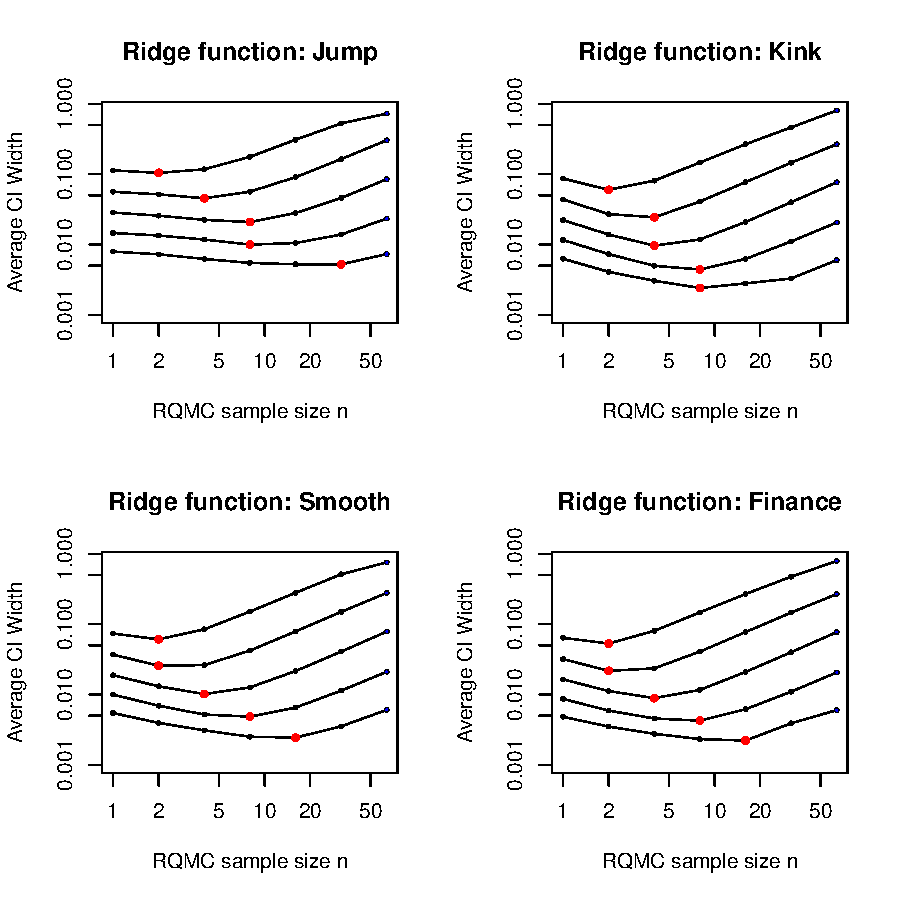
\includegraphics[width=0.9\linewidth]{figmeanwidths}
    \caption{
Mean confidence interval width for the betting method
as a function of the RQMC sample size $n$.
There is one panel for each of the $4$ ridge functions.
Within a panel the curves are for $N=2^{2r}$
for $r=4,5,6,7,8$ from top to bottom. The smallest
mean width for each $N$ is marked with a larger circle.
The means are taken over all $20$ replicates and
all $4$ dimensions used.
    }
    \label{fig:meanwidths}
\end{figure}

We see in Figure~\ref{fig:meanwidths} some things that
align very well with our analysis and some that
were not anticipated.
The optimal samples sizes $n$ are very small and
they grow slowly with the budget $N$ as expected.
The least smooth ridge function $g_\jmp$ has
the fastest growing $n$ as expected.
The interval widths for $g_\fin$ and $g_\smo$
were very close to each other 
%and those two ridge integrands had identical optimal $n$
despite having very different smoothness
and then they had identical optimal $n$ at each $N$.
For $N=2^{10}$ the optimal $n$ for $g_\knk$
is larger than the one for $g_\smo$ as expected
but at $N=2^{16}$, it is $g_\smo$ that has
the larger optimal $n$.

Our expectations were based on asymptotic
considerations.
First, we used the fact that the betting interval
widths asymptotically approach the optimal
empirical Bernstein widths from Bennett's
inequality.  Second, we supposed that the RQMC variance
is asymptotic to $\sigma_0^2n^{-\theta}$ apart from logarithmic
factors. We also used the finite sample Bennett
widths from~\eqref{eq:benh} \art{because
the asymptotic expression $\sigma_n\sqrt{2\log(2/\alpha)/R}$
does not have a meaningful optimum.}
The empirical results strongly confirm our
asymptotic findings that small $n$ is best overall,
but among such small $n$, it is less clear
how to choose $n$ based on smoothness of $f$.

\subsection{Functions with known RQMC variance}

In some simple settings we can compute the
RQMC variance exactly (i.e., non-asymptotically)
for a specific value of $n$.
This allows us to directly
compare the widths of the betting intervals to
the value we get from Bennett's formula. We know
that the betting intervals have that length
asymptotically matches Bennett's formula, but
we also want to study how that length
approaches Bennett's formula in some examples.
We choose one smooth function with $\theta=3$
and one discontinuous function with $\theta=2$.
Both of them have dimension $d=1$.

For $d=1$ and a nested uniform scramble of $n=2^k$ Sobol'
points we know that 
\begin{align}\label{eq:varsobol1d}
\var(\hat\mu) =\frac1{n^2}\sum_{\ell=1}^n\var( f(x_\ell))
\end{align}
where $x_\ell\sim\dunif[(\ell-1)/n,\ell/n]$ are independent.
The smooth function we choose is $f(x)=xe^{x-1}$.
We know that $\var(\hat\mu)\asymp (5-e^{-2})/(48n^3)$
for this function.
For exact computations we have
\begin{align}\label{eq:varonesmooth}
\var(f(x_\ell))=n\int_{(\ell-1)/n}^{\ell/n}f(x)^2\rd x
-\Bigl(n\int_{(\ell-1)/n}^{\ell/n}f(x)\rd x\Bigr)^2
\end{align}
which can be computed for finite $n$ using the closed form antiderivatives of $f$ and $f^2$.  Using~\eqref{eq:varonesmooth}
in~\eqref{eq:varsobol1d} we get a value that increases
rapidly towards the asymptotic expression but differs
meaningfully for $n\le 8$.
The discontinuous function we choose is $f(x)=1\{x<1/3\}$
from Section~\ref{sec:semiempirical}.
It has $\var(\hat\mu)=2/(9n^2)$.

Using the known variances, we can compute the
half width from Bennett's inequality ~\eqref{eq:bennettwidth}
for our $\sigma^2_n$ and $R=N/n$ double it
and then divide the average betting width
by this value. The results are in shown  in Figure~\ref{fig:widthstoeb}. For our two example
functions we see that as $R=N/n$ increases (so $n$ decreases
for fixed $N$)
the ratio of widths decreases and approaches the
theoretically expected value of $1$.
At the smallest $R$ (largest $n$) the betting
intervals were two or three times as wide as the
Bennett intervals for the discontinuous function.
They were somewhat wider for the smooth function.

\begin{figure}[t]
    \centering
    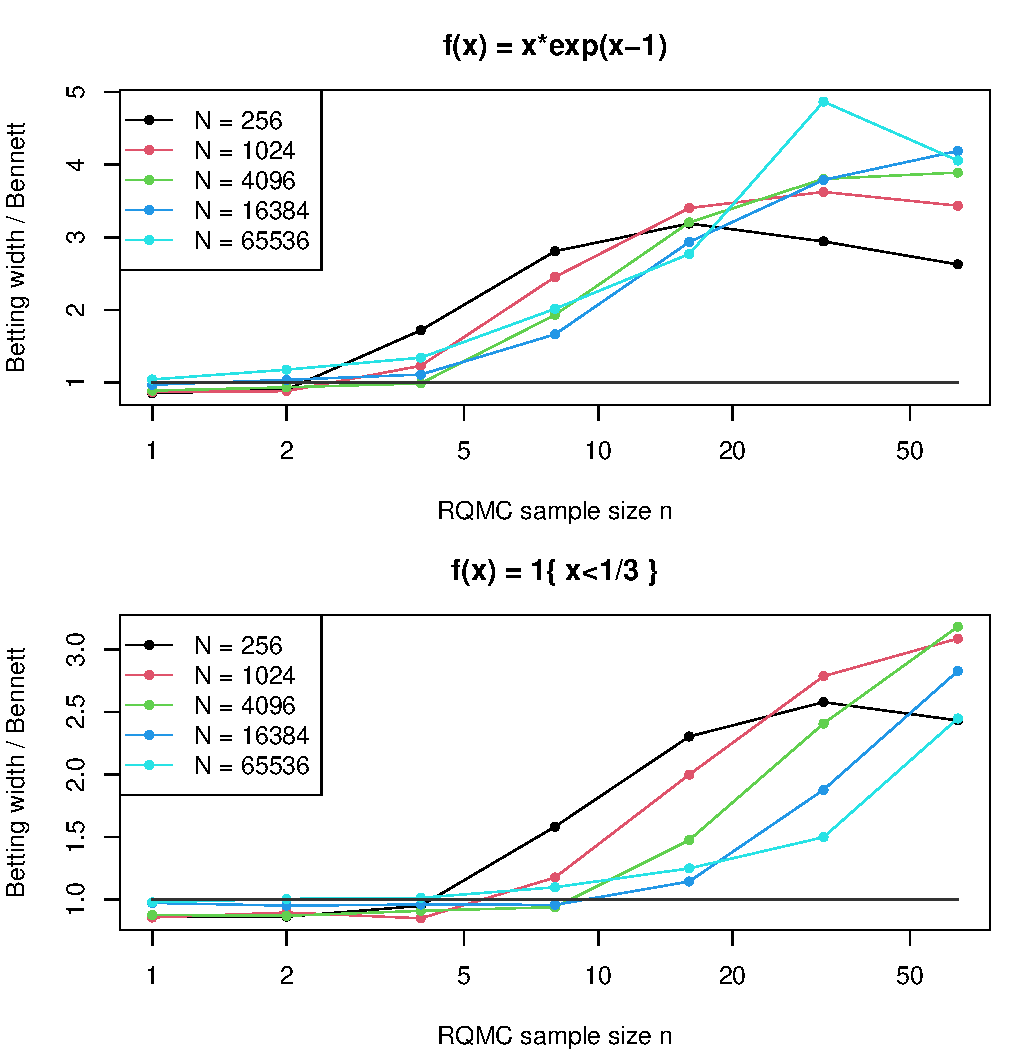
\includegraphics[width=1.\linewidth]{figwidthstoeb}
    \caption{Caption}
    \label{fig:widthstoeb}
\end{figure}

The betting windows are computed without knowledge
of the exact variance $\sigma^2_n$ that the Bennett
interval uses.  They are instead based on estimates
of that variance and they must therefore allow for
uncertainty in the variance estimate.  It is then not
surprising that the resulting intervals are wider
than the Bennett ones. \art{We see in Table~\ref{tab:benvsbetn} that
the hedged betting intervals' minimum lengths were
not found at larger $n$ than the minimizers
of the Bennett intervals. They were either equal
or half as large as $n_*$.}


\begin{table}
\centering
\begin{tabular}{rrr}
\toprule
$N$ & $n_*$ & $n_{\mathrm{opt}}$\\
\midrule
256 &  4   & 4\\
1,024&  8   & 4\\
4,096 & 8   & 8\\
16,384 & 16 & 16\\
65,536 & 32 & 16\\
\bottomrule
\end{tabular}
\caption{\label{tab:benvsbetn}
For the given budgets $N$, we show $n_*$ as the
minimizer of the Bennett width \eqref{eq:benh} 
over $n=2^k$ for integer $k$, for the function
$f(x) = 1\{x<1/3\}$. Then $n_{\opt}$ is
the value of $n$ that minimized the average
width of the hedged betting confidence interval
for the given $N$.
}
\end{table}

\art{[I don't see a role for the two dimensional
discontinuous function after what we have 
learned from the ridge functions and exact
variance functions.]}

\section{Discussion}\label{sec:discussion}

In favorable cases
the RQMC variance is $\tilde O(n^{-3})$ and then
using a fixed number $R$ of replicates of
point sets with $n\to\infty$ we can estimate
the integral $\mu$ with a standard deviation 
of $\tilde O(N^{-3/2})$ for $N=nR$ along with
an unbiased estimate of the variance of that estimate.
It remains very difficult to get a confidence 
interval of width $\tilde O(N^{-3/2})$ \cite{err4qmc}.
Using Student's $t$ with a small $R$ gave good
results in an extensive simulation by \cite{LEcEtal24a}
but that success is not yet theoretically understood.
For an integrand subject to known bounds, we can get
a non-asymptotic confidence interval by using $R$
replicates of $n$ RQMC points using a
predictable plug-in empirical Berstein confidence
interval.  In that approach the optimal $n$
grows proportionally to $N^{1/(\theta+1)}$ and
the resulting confidence intervals have width
$O(N^{-\theta/(\theta+1)})$.
It remains to find a reliable way to choose $n$
empirically. 

It also remains to find a good way to
use RQMC in confidence sequences as opposed
to confidence intervals.   We might
set up $R$ independent infinite sequences of RQMC
points and then stop them at the first $n$
where they provide a $1-\alpha$ interval
narrower than some $\epsilon$.  In a task
like that it makes sense to only use
$n=2^k$ for integers $k$. 
That is partly because powers of two are good
for scrambled Sobol' points, but also because
in RQMC it is generally advisable to study
sample sizes $n$ that grow geometrically
not arithmetically \cite{sobo:1998}.  The
idea is that if $n$ is not large enough to get
a good answer, then $n+1$ is unlikely to be
much of an improvement.
A confidence sequence based on geometrically
growing $n$ would not have to be as wide as one for arithmetically
growing $n$.

\art{For scrambled Sobol' points it is strongly
advisable to take $n=2^k$ because those are
the best sample sizes and they can even give
a better convergence rate. The Halton sequence \cite{Hal60} does
not have strongly superior sample sizes and so $n$ need
not be a power of two for it.  The 
two scrambles we considered for Sobol' points can
also be applied to the Halton sequence getting
$\var(\hat\mu)=o(1/n)$ without requiring special
sample sizes $n$ \cite{haltongain}.
There are however no published non-trivial settings
where scrambled Halton points can obtain $\theta>2$.
}


% \fred{[Since the practical value of $n$ is small, should we mention that low discrepancy points are typically constructed for large $n$, and that specialized constructions that admit randomizations might be useful?  I doubt that we could get very specific.]}\art{[I don't think so. We still need unbiasedness, so we would have to randomize those special constructions.  I was planning to mention scrambled Halton here at the very end.  Then you don't have special sample sizes $n$, but there are also no known non-trivial settings with $\theta>2$. I didn't want to carry that through the whole paper because it would be hard for a non-QMC person to follow.]}

\section*{Acknowledgments}

We thank Aaditya Ramdas and Ian Waudby-Smith for helpful
discussions and for the \art{xxx} software
from \art{xxx} that we used.
ABO was supported by the U.S.\ National Science Foundation
grant DMS-2152780.

\art{TODO: We need tidy up references: capitalizations,
consistent name vs initials.}

\bibliographystyle{plain}
\bibliography{FJH25,FJHown25,ebci4rqmc}

\end{document}